%%%%%%%%%%%%%%%%%%%%%%%%%%%%%%%%%%%%%%%%%%%%%%%%%%%%%%%%%%%%%%%%%%%%%%%%%%%%
%% Working title: Social Network Analysis of Twitter Topic-Network Structures during the 2019 European Elections
%% Andrea Domenico Antonacci, a.d.antonacci@tilburguniversity.edu
%% January 2020
%%%%%%%%%%%%%%%%%%%%%%%%%%%%%%%%%%%%%%%%%%%%%%%%%%%%%%%%%%%%%%%%%%%%%%%%%%%%
\RequirePackage{amsmath} % Load amsmath first
\documentclass[a4paper,12pt]{article}
% Set margins
\usepackage[margin=1in]{geometry}
% Set language
\usepackage[russian,greek.ancient,english]{babel}
\usepackage[utf8]{inputenc}
\usepackage[T2A,OT2,T1]{fontenc}
\DeclareTextFontCommand{\textcyr}{\cyr}
% Define fonts
\usepackage{tempora} % Used for special characters not available in mainfont
% \usepackage{gfsdidot} % Use Didot font
\usepackage{mathpazo} % Or use Palatino font
% Set line spacing
\renewcommand{\baselinestretch}{1.5}
% Allow multi-column environments
\usepackage{multicol}
\setlength\columnsep{40pt}
% Formulas and math
\usepackage{amssymb}
\usepackage{algorithm} % For algorithms
\usepackage{algpseudocode}
\usepackage{units} % Allow nice in-line, diagonal fractions
% Define bibliography
\usepackage[authoryear]{natbib}
\bibliographystyle{apa}
% Allow hyperref with click-through sections and references
\usepackage[unicode=true,pdfusetitle,bookmarks=true,bookmarksnumbered=true,bookmarksopen=true,bookmarksopenlevel=1,breaklinks=false,pdfborder={0 0 0},pdfborderstyle={},backref=false]{hyperref}
\hypersetup{pdfpagelayout=OneColumn, pdfnewwindow=true, pdfstartview=XYZ, plainpages=false,pdfauthor={Andrea Domenico Antonacci},colorlinks=true,linkcolor=ForestGreen,citecolor=ForestGreen}
% Allow fancy headers
\usepackage{fancyhdr}
\fancypagestyle{SectionFirstPage}{\fancyhead{}\renewcommand{\headrulewidth}{0pt}} % Use this pagestyle to hide headers on the first page of sections
\renewcommand{\floatpagefraction}{.9}% Set the amount of figures for floatpages
% Misc packages
\usepackage{setspace} % To set line spacing locally
\usepackage{graphicx} % Allow figures
\graphicspath{ {images/} }
\usepackage{lipsum} % For prototyping
\usepackage[dvipsnames]{xcolor} % Enable more colors in text
\usepackage{microtype} % Improve justification
\usepackage{url} % Line-breaking urls
\usepackage{pdflscape} % Allow pages in landscape mode
\usepackage{multirow} % Allow multirow in tables
\usepackage[labelfont=bf]{caption} % Set caption distances from tables and figures
\usepackage{subcaption} % For subfigures
\captionsetup[table]{skip=10pt, position=top}
\captionsetup[figure]{belowskip=10pt, skip=5pt, position=top}
\usepackage[nottoc]{tocbibind}
\usepackage{makecell} % Allow to break lines inside a table cell
\usepackage[para]{threeparttable}
\usepackage{rotating}
\usepackage{textcomp} % For symbols
\usepackage{tikz} % For graphs and graphics
\usetikzlibrary{shapes.geometric, shapes.misc, arrows, positioning}
\def\checkmark{\tikz\fill[scale=0.4](0,.35) -- (.25,0) -- (1,.7) -- (.25,.15) -- cycle;} % Define a checkmark (tick)
\tikzstyle{startstop} = [rectangle, rounded corners, minimum width=3cm, minimum height=1cm,text centered, draw=black]
\tikzstyle{io} = [trapezium, trapezium left angle=70, trapezium right angle=110, minimum width=2cm, minimum height=2cm, text centered, text width=2.5cm, draw=black]
\tikzstyle{process} = [rectangle, minimum width=3cm, minimum height=1cm, text centered, draw=black]
\tikzstyle{decision} = [diamond, minimum width=3cm, minimum height=1cm, text centered, draw=black]
\tikzstyle{arrow} = [->,>=triangle 45]
\usepackage{varioref} % Intelligent references with pageref automatically added

% Define title page
\usepackage{titling}
\renewcommand\maketitlehooka{\null\mbox{}\vfill} % To vertically center it
\renewcommand\maketitlehookd{\vfill\null}
\title{Social Network Analysis of Twitter Topic-Network Structures during the 2019 European Elections}
\author{Andrea Domenico Antonacci, SNR 2032465}
% \date{October 2019} % Uncomment for custom date
% \global\hyphenpenalty=100000 % avoid hyphenation globally, for debug only

%%%%%%%%%%%%%%%%%%%%%%%%%%%%%%%%%%%%%%%%%%%%%%%%%%%%%%%%%%%%%%%%%%%%%%%%%%%%
%% Content below
%%%%%%%%%%%%%%%%%%%%%%%%%%%%%%%%%%%%%%%%%%%%%%%%%%%%%%%%%%%%%%%%%%%%%%%%%%%%
\begin{document}

% Title page
{ % Use curly brackets to create a group and assign properties locally
\setstretch{1.0}
\maketitle\thispagestyle{empty}
\vspace{1cm}
{\large {Master Thesis in Marketing Management\par Tilburg School of Economics and Management\par Tilburg University\par}}
}
\vspace{1cm}
{
\setstretch{1.0}
\begin{multicols}{3}
\raggedright
Supervisor:\\Second reader:
\vfill\null
\columnbreak
dr. Hannes Datta\\Nazli Alagöz
\vfill\null
\columnbreak
Associate Professor\\Ph.D. Candidate
\end{multicols}
}

% TOC
{ % Use curly brackets to create a group and assign properties locally
\newpage
\setstretch{1.0}
\hypersetup{linkcolor=black} % Links in TOC are black
\pagenumbering{roman}
\tableofcontents
}

% Abstract
\newpage
\begin{abstract}
\addcontentsline{toc}{section}{Abstract}
This paper explores how Twitter users differently interact based on the topic of discussion in online conversations. For this purpose, we employ concepts of Social Network Analysis to examine how node-level network topology measures may affect the likelihood of interaction and the extent to which two nodes interact in distinct topic-network structures. We collect 21 million sampled tweets via the Twitter API, tracking more than 700 keywords during the 2019 European Elections. We perform our analysis on a final data set of 2,259,717 tweets on five politics-related topics. We find systematic differences in the direction of the effect of centrality measures between distinct topics of discussion, but not for degree and clustering metrics. Notably, the target user’s eigencentrality positively predicts the interaction between users, regardless of the topic. However, among the pairs of interacting users, the direction of this effect varies between topics. We also show that the sender’s eigencentrality negatively influences the probability of interaction, but not the extent to which users interact between them.
\end{abstract}

% Content
\newpage
\pagestyle{fancy} % Initiate headers
% Define global headers for all the sections
\lhead{\nouppercase{\rightmark}}
\rhead{}
\pagenumbering{arabic}
\section{Introduction}\label{Introduction}\thispagestyle{SectionFirstPage} % Hide headers on the first page of the section
The rise of synchronous computer-mediated communication (CMC) in the last decades allowed for instant sharing and access to worldwide information, which profoundly revolutionized social activity and human interaction on the Internet. Ideas, political messages, tweets, memes, and advertisements spread today on the Internet within enormous networks of nodes and edges. Using online social networks services (OSN), individuals can choose whom to engage with, constructing their own network of interactions. Albeit recommendation algorithms have taken hold in the recent years, users still actively select their information sources. This process varies according to the way the social network platform is designed – e.g., by following, subscribing, sharing, etc. – yet its rationale is almost universal.

Many recent studies on social network analysis (SNA) document these patterns of interaction. Central issues of particular interest range from the evolution of interaction behavior in social networks over time \citep[e.g.,][]{mulder:2019} to the role of message in viral marketing campaigns \citep[e.g.,][]{liu-thompkins:2012} and Twitterstorms phenomena \citep[e.g.,][]{timm:2016}.
Researchers have extensively studied single network characteristics – i.e., tie strength, centrality, and density measures, to name a few – to classify users and explain information diffusion at the individual level in social networks \citep{granovetter:1973, borgatti:2005}.
In fact, SNA has been applied to OSN in many fields, from studying the influence of word of mouth on new product launches \citep[e.g.,][]{deer:2019} to sexual relationships and couple formation \citep[e.g.,][]{ortega:2017}. While these approaches have proven successful, a deeper understanding of information diffusion at the network level can only be achieved when taking multiple measurements jointly \citep{himelboim:2017}.

This appears of utmost relevance in the light of the prominent influence that OSN exert on the public opinion nowadays \citep{kwak:2010, lerman:2010}. For instance, it might be especially worth studying how OSN are displacing more traditional media outlets during political election campaigns \citep[see, e.g.,][]{hemsley:2019, buccoliero:2020, kruikemeier:2014}.
In fact, many academics have carried out studies about the political discourse in the context of OSN, the majority of which mainly focused on two concerns: which users are the most ``influential'' (key-members identification) and how information flows throughout the network \citep[as cited in][]{bode:2016}. Previous work on information diffusion and key-members identification in social networks has been traditionally based on centrality measures \citep{freeman:1978}. However, we believe that further investigation is needed to better grasp how network characteristics, such as centrality, differ per topic in online conversations.
% no citation

In this paper, we argue that the above-mentioned network-level measurements may systematically differ among topics of conversation on OSN. We are of the view that analyzing such topic-network structures might help to better understand information dissemination. We ground our work on political conversations because of their intrinsically polarizing, and easily identifiable topics. More specifically, we focus on the 2019 European Election event because of its presence in multiple countries. Twitter can be considered suitable for these research purposes. First, as one of the foremost social network platforms that is globally used and steadily growing, it established itself as one of the most popular online political arena \citep{tumasjan:2011} and empowered politicians to share their messages broadly without the need of journalists \citep{blumler:2001}. Moreover, by providing open access to its API – with a free tier available too – it offers researchers an unprecedented opportunity to easily collect data. The retweet feature allows its users to spread information beyond the reach of their original followers, and therefore enables us to clearly reconstruct the conversation trees. Lastly, \citet{Toubia:2013} also showed that Twitter's design pushes its users to voluntarily contribute with content because of the intrinsic utility and the image-related utility, de-facto disclosing their personal information, thoughts, and experiences by tweeting, and thus providing a constant and sheer volume of data.
% because of the image utility and ... utility hypotheses?
In this study, we collect more than 20 million tweets on the 2019 European Parliament election, over the entire electoral period, from one week before (May 16, 2019) up to more than a week after the elections in all the Member States. This is a \emph{sample} of the stream of tweets in that time period, resulted from the tracking of approximately 700 different keywords\footnote{A complete list of tracked keywords can be found in the Appendix section.} via the Twitter real-time filter API\footnote{Twitter's APIs and their limitations will be thoroughly discussed in section \ref{Data}.}. We track eleven politics-related topics, chosen because of their relevance and omnipresence in most countries, with the following keywords\footnote{All the keywords have been accordingly translated into all the different languages spoken in the European Union.}: \texttt{brexit}, \texttt{eu institutions}, \texttt{fake news}, \texttt{gender equality}, \texttt{lgbt rights}, \texttt{populism}, \texttt{public debt}, \texttt{refugees}, \texttt{single market}, \texttt{terrorism}, \texttt{unemployment}.
Subsequently, we select our data to retain only contributing users to a given topic – i.e., users whose tweets initiated a conversation, as well as their retweets, replies, and @-mentions. We construct topic-network structures by obtaining nodes and edges for each topic, and calculate a set of network measurements via Gephi 0.9.2\footnote{Gephi is a visualization and exploration software for graphs and networks that is open-source and free: \url{https://gephi.org/}.}. We propose three generalized regression models to explain how information flow characteristics differ among topics, and apply them to four different topic-networks. We find evidence for systematic differences in the direction of the effect of centrality measures between distinct topics of discussion, but not for degree and clustering metrics.

Therefore, this paper will be structured as follows: in section \ref{Literature} we deepen into the extant literature. Our data collection and modeling methodology is outlined in section \ref{Data}. In section \ref{Models}, we explain our models and analysis. In section \ref{Results}, we discuss the results. Section \ref{Discussion} concludes this paper.

\section{Literature Review}\label{Literature}\thispagestyle{SectionFirstPage} % Hide headers on the first page of the section

% \subsection{Related Work on Social Network Topology}
A vast body of research has focused on SNA applied to online social networks. Because of the nature of this paper, we put emphasis on three streams of literature that deal with the topological analysis of social networks, while we neglect the numerous studies devoted to other disciplines – e.g., linguistics, mostly focused on text analysis, user generated content, etc. Our classification of the current literature is summarized in Table \vref{literature-overview}.

The first group of studies addresses information diffusion, namely how information propagates throughout the network. Many articles in this group focus on the issue of social influence, that is the change in behavior of individuals attributable to other actors in a network. The strength of such social influence may depend on many factors, such as tie strength, the distance between users in the network, etc. \citep{aggarwal:2011}.
For instance, researchers in this group use Twitter data to investigate the influence of word of mouth (WOM) on consumer demand for new products \citep{deer:2019}, as well as social influence of important actors – called middle-level gatekeepers, who have between 1,800 and 26,000 followers on Twitter – in the spreading of viral events \citep{hemsley:2019}.
Similarly, \citet{aral:2007} show how demographics, network factors, functional relationships, and the strength of ties influence the diffusion of news, compared to the diffusion of discussion topics. They find that, while demographic and network factors always heavily influence diffusion, tie strength only does so in the diffusion of discussion topics. Unfortunately, this study is based on email data and the question remains on whether the same conclusions apply to other OSN, such as social media platforms like Twitter. \citet{lerman:2010} conduct a similar study on news propagation based on Digg and Twitter data sets, but without controlling for the effect of network factors such as centrality. Likewise, \citet{liu-thompkins:2012} concentrates on seeding strategies to spread viral messages and shows that choosing highly influential users with strong ties is a better strategy than simply opting for a wider reach. Lastly, \citet{zhang:2013} model the propagation probability based on topic relevance to the target message, although without controlling for the effect of network metrics. Unfortunately, all the approaches adopted by this group of studies are limited in showing the interaction of topics and network factors.

The second set of papers deals with community identification in OSN. Studies on community detection highlight the structure of relationships in the network and identify the users with a particular position. For instance, \citet{grandjean:2016} tries to answer to the question of ``who's following who?'' in a descriptive network analysis. Similarly, \citet{java:2007} document users intentions associated in a community and find that users with similar intentions tend to connect more with each other. \citet{zhao:2012} take a step closer to the analysis of topic-network structures and propose a topic-oriented community detection approach. However, a gap remains in our knowledge regarding how these topical clusters differ on a network metrics basis, and whether such differences can be explained and uniquely attributed to the distinct topics of discussion on online social media platforms.

The third stream of research, in which we position our own work, examines topic-network structures in the context of OSN. These studies center around the spreading of topics through the graph, taking into account different network factors and tracking the structure of information spread as if it was an ``infection'''s growth, drawing inspiration from epidemiological studies.
\citet{ardon:2013} perform a large scale measurement study, observing temporal, spatial, and geographical evolution of both popular and less popular topics. However, their approach remains topic-centered and does not investigate the interaction of users. % from topic pov. --> dv is not interaction of Users, but topic diff
One method to address this issue is to model the strength of topic-level direct and indirect influence between nodes in a network, and later apply it to predict user behavior \citep{liu:2010, tang:2009, lim:2016}.
Some researchers adopt a different approach and, instead of relying on hashtags, they infer the topics of discussion from a text analysis, where an unsupervised machine learning technique is used to identify latent topic information \citep{hong:2010, lhuillier:2011}. Unfortunately, these studies cannot be taken as evidence for the existence of a causal link between the differences in network measures and the interacting topics of discussion.
There are several ways of handling this problem. Many scholars tried to characterize information diffusion in entire networks using a single network measurement only - e.g., density, or centrality.
\citet{himelboim:2017} recognize the pitfall and overcome this difficulty by classifying Twitter conversations based on multiple network-level measurements and patterns of information flow. In fact, the authors claim that to gain insights on information flow for the whole network it is crucial to integrate single network-level measurements with one another. Nevertheless, their findings do not imply that the observed differences can be uniquely attributed to the distinct topics in question, as no causal relationship is assessed.

The contribution of this paper to the literature is twofold. First, we aim at reconstructing topic-network structures to subsequently test the differences of multiple network-level measurements among topics with three generalized linear models. As a second contribution, we propose an easily reproducible methodology for data collection and modeling, that could serve as a blueprint for similar large-scale social network analyses, and facilitate the replication of a real-time data collection and visualization environment.

\newpage
\thispagestyle{SectionFirstPage}
\renewcommand{\arraystretch}{1.2}
\begin{sidewaystable}
  % \setlength\extrarowheight{1pt} % provide a bit more vertical whitespace
  \centering
  \footnotesize
  \captionsetup{size=footnotesize}
  \caption{Current literature overview of topological SNA applied to online social networks.\label{literature-overview}}
  \begin{threeparttable}
  \begin{tabular}{ l c c c c c c c c }
    \hline
    \multirow{2}{*}{Paper} & \multicolumn{4}{c}{Effect of} & \multirow{2}{*}{Outcome measure(s)} & \multirow{2}{*}{Topic(s) control} & \multirow{2}{*}{Text data} & \multirow{2}{*}{Data size} \\
    & degree & tie strength & centrality & clustering & & & & \\
    \hline
    \multicolumn{9}{l}{\textit{Information diffusion}} \\
    \citet{aral:2007} & & \checkmark & \checkmark & & information awareness & \checkmark & & 125,000 emails \\
    \citet{deer:2019} &  &  &  &  & consumer demand for movies & & \checkmark & 50M tweets \\
    \citet{hemsley:2019} &  &  &  &  & information spreading &  &  & 11,000 tweets \\
    \citet{lerman:2010} & \checkmark &  &  &  & information spreading & \checkmark &  & 137,582 Twitter users \\
    \citet{liu-thompkins:2012} & \checkmark & \checkmark &  &  & \# of views per video & &  & 101 YouTube videos \\
    \citet{timm:2016} & \checkmark &  & \checkmark &  & –\textsuperscript{a} & \checkmark & \checkmark & 51,000 tweets \\
    \citet{zhang:2013} & \checkmark &  &  &  & propagation probability & \checkmark &  & 10,892 Twitter users \\
    \multicolumn{9}{l}{\textit{Community identification}} \\
    \citet{grandjean:2016} & \checkmark &  & \checkmark &  & –\textsuperscript{b} &  &  & 2,500 users \\
    \citet{java:2007} & \checkmark &  &  &  & –\textsuperscript{b} &  &  & 76,177 users \\
    \citet{zhao:2012} & \checkmark & \checkmark &  &  & purity of topics in community & \checkmark &  & \makecell{275,332 emails,\\1,490 webblogs,\\2,708 papers} \\
    \multicolumn{9}{l}{\textit{Topic-network structures}} \\
    \citet{ardon:2013} & \checkmark &  & \checkmark & \checkmark & topic popularity & \checkmark &  & \makecell{10M users,\\5.96M topics} \\
    \citet{himelboim:2017} &  &  & \checkmark &  & –\textsuperscript{c} & \checkmark &  & 60 topics \\
    \citet{hong:2010} &  &  &  &  & –\textsuperscript{d} & \checkmark & \checkmark & \makecell{1,992,758 tweets,\\514,130 users} \\
    \citet{lhuillier:2011} &  &  & \checkmark &  & –\textsuperscript{d} & \checkmark & \checkmark & 29,057 posts \\
    \citet{lim:2016} &  &  &  &  & –\textsuperscript{e} & \checkmark &  & \makecell{60,370 +\\781,186 tweets} \\
    \citet{liu:2010} & \checkmark & \checkmark &  &  & influence strength & \checkmark &  & 40,000 users \\
    \citet{tang:2009} & \checkmark & \checkmark &  &  & interacted, \# of interactions & \checkmark &  & \makecell{2,329,760 papers,\\640,134 authors,\\18,518 films} \\
    % Is tang et al on interacted and no of interactions?
    \textsc{This paper} & \checkmark &  & \checkmark & \checkmark & interacted, \# of interactions & \checkmark &  & 21,337,037 tweets \\
    \hline
    % \textit{Note:}  & \multicolumn{8}{r}{{*}They used an agent-based actor model to run a social simulation;} \\
    % & \multicolumn{8}{r}{{**}They applied algorithms such as Clique Percolation Method (CPM) to find overlapping communities.} \\
    % & \multicolumn{8}{r}{{***}They used the Clauset–Newman–Moore clustering algorithm included in the NodeXL package.} \\
  \end{tabular}
  \begin{tablenotes}
\item[a]{They use an agent-based actor model to run a social simulation.}
\item[b]{They apply algorithms such as Clique Percolation Method (CPM) to find overlapping communities.}
\item[c]{They use the Clauset–Newman–Moore clustering algorithm included in the NodeXL package.}
\item[d]{They use the Latent Dirichlet Allocation technique to run a text analysis.}
\item[e]{They use hierarchical Poisson-Dirichlet processes (PDP) for text modeling.}
\end{tablenotes}
\end{threeparttable}
\end{sidewaystable}
% 1 paper
% 2 degree
% 3 tie strength
% 4 centrality
% 5 clustering
% 6 outcome measure
% 7 per topic
% 8 text data
% 9 data size
% 10 Modeling

\section{Data and Methodology}\label{Data}\thispagestyle{SectionFirstPage} % Hide headers on the first page of the section
\subsection{Research Design}
We are interested in assessing how Twitter network structures differ among distinct topics of discussion. We explore the differences between such topic-network structures in terms of their network topology measures and how these affect the number of interactions between pairs of users. For this purpose, we first need to collect the data and retrieve tweets conversations based on selected topics. Next, we perform a regression analysis on these networks, where the predictors are the nodes' respective network measures, and the explained variable is the number of interactions between every pair of nodes in the network.
Before explaining our methodology in more detail, we set out some basic definitions of fundamental concepts of graph theory and social network analysis.

A social network is a network (or graph) of \textit{interactions} or \textit{relationships} between actors \citep{aggarwal:2011}. The actors are called \textit{nodes}, whereas their interactions are called \textit{edges}, links, or ties. Social networks are not restricted to a purely online form. In fact, they have been studied by sociologists for generations before the advent of OSN \citep[see, e.g.,][]{milgram:1967}. However, in the context of OSN, users are often the nodes who form ties or connections (edges) among themselves to exchange content like text, images, videos, or in another form. In this paper, the nodes represent the interacting users and the edges their tweets, retweets, mentions, or replies.

\begin{figure}[ht]
\centering{}\caption{Nodes and edges in undirected and directed graphs.\label{fig:directed-undirected}}
\begin{center}
\begin{tikzpicture}[scale=1.5]
    \node[shape=circle, draw=black, minimum size=0.9cm] (i) at (1,2) {$i$};
    \node[shape=circle, draw=black, minimum size=0.9cm] (j) at (0,0) {$j$};
    \node[shape=circle, draw=black, minimum size=0.9cm] (k) at (2,0) {$k$};

    \path [-](i) edge node[left=4pt] {$e_{i,j} = e_{j,i}$} (j);
    \path [-](j) edge node[below=4pt] {$e_{j,k} = e_{j,k}$} (k);
    \path [-](k) edge node[right=4pt] {$e_{k,i} = e_{i,k}$} (i);

    \node[shape=circle, draw=black, minimum size=0.9cm] (i) at (5,2) {$i$};
    \node[shape=circle, draw=black, minimum size=0.9cm] (j) at (4,0) {$j$};
    \node[shape=circle, draw=black, minimum size=0.9cm] (k) at (6,0) {$k$};

    \path [->,>=triangle 45](i) edge node[left=4pt] {$e_{i,j}$} (j);
    \path [->,>=triangle 45](j) edge node[below=4pt] {$e_{j,k}$} (k);
    \path [->,>=triangle 45](k) edge node[right=4pt] {$e_{k,i}$} (i);

    \node[shape=circle, draw=none] (label1) at (1,-1) {Undirected graph};
    \node[shape=circle, draw=none] (label2) at (5,-1) {Directed graph};
\end{tikzpicture}
\end{center}
\vspace{-60pt}
\end{figure}

A network can be \textit{directed}, like follow relationships on Twitter, or \textit{undirected}, like mutual friendships on Facebook (see Figure \vref{fig:directed-undirected}). In directed graphs, asymmetric binary relations may occur, hence the edge from node $i$ to node $j$ is different than the one from $j$ to $i$. Moreover, a network may be \textit{weighted}, where a weight is set for each edge or, whenever multiple edges can occur between two nodes (e.g., in a conversation of tweets), the weight can be the number of edges between these nodes.
In our case, in a weighted graph $\mathcal{G}$, let $e_{i,j}$ be the edge between node $i$ and node $j$, and let $w_{i,j}$ be the weight on edge $e_{i,j}$ computed as the number of interactions between $i$ and $j$. The total weight $w_i$ of the node $i$ can be thus defined as the sum of weights of all its edges, that is $w_i = \sum_{k=1}^{d_i} w_{i,k}$, where $d_i$ denotes its degree. The \textit{degree} of a node is defined as the number of edges for that given node – i.e., how many connections a node has in the network. The weighted degree is similarly based on the number of edges for that node, but ponderated by the weight of such edges – i.e., the number of interactions between a pair of nodes.
One final notable network concept is related to \textit{density}, which stands for the proportion of edges present in a network compared to the number of all potentially possible edges - i.e., the completeness of a network. Density is therefore defined as
${Network\, Density = \frac{No.\, of\, actual\, edges}{No.\, of\, potential\, edges} = \frac{No.\, of\, actual\, edges}{\frac{N\; (N-1)}{2}}}$,
where $N$ is the total number of nodes in the network.

To perform our study, we require nodes and edges tables for each topic of discussion. The former are tables with data for each node, while the latter contain information on the edges between each pair of nodes. In our case, nodes tables include network topology measures for each node, while edges tables specify which are the source and target nodes, and the weight of their edge. We provide examples of the structure of these tables in Appendix \vrefrange{nodestable}{metricstable}.

The process to obtain the final data set for each topic consists of four main sequential stages.
First, primary data is collected in real-time via the Twitter API endpoints, then stored on a MongoDB (NoSQL) database for real-time querying and visualization, as well as on an Amazon Web Services (AWS) S3 bucket for long-term storage.
Secondly, data is cleaned, selected, and prepared with a five-step pipeline in Python. These scripts transform the raw data set into nodes and edges tables for each analyzed topic.
Subsequently, the latter tables are imported to Gephi in order to visualize their graph structures and compute network measurements.
Lastly, we import into an R program the updated tables with new measures exported from Gephi. This R script constructs adjacency lists and runs three generalized linear models for each topic, where the covariates are node-level network metrics. First, we run a multiple regression model on the number of interactions for every pair of users. Secondly, a logistic model to assess the probability of interaction between two users. Finally, a conditional (filtered) multiple regression model on the number of interactions, only for those pairs of users that interacted with each other.

In this chapter, we further illustrate the rationale behind each step in the pipeline. To enable reproducibility of our research, we publish all our scripts on GitHub with open access\footnote{The repository can be accessed from: \url{https://github.com/andreantonacci}.}.
% Too short
\subsection{Data Collection}
\subsubsection{Twitter Real-time Filter API}
We conduct all the analyses in this paper on primary data collected via the Twitter real-time filter API\footnote{\url{https://developer.twitter.com/en/docs/tweets/filter-realtime/overview}.} (standard plan) – or streaming API. We commence the collection of data on May 16, 2019, at 12:50:00 UTC, using the \texttt{tweepy}\footnote{\url{https://www.tweepy.org}.} library for Python to access the Twitter API.

The API returns public tweets that match one or more filters (e.g., a keyword, hashtag, username, or location) in a JSON response format\footnote{A full list of JSON tweet objects and a tweet data dictionary can be found here: \url{https://developer.twitter.com/en/docs/tweets/data-dictionary/overview/tweet-object}.}. The latency from the tweet publication to its delivery on the API is typically within seconds. The default access level (standard plan) to the Twitter API is free but subject to some limitations: it allows for tracking up to 400 keywords and returns at most 1\% of all tweets being published on Twitter at a given moment \citep{morstatter:2014}. Because of the limited resources available for this project, we cannot set up an enterprise plan and utilize the PowerTrack API\footnote{\url{https://developer.twitter.com/en/docs/tweets/filter-realtime/overview/powertrack-api}.}, which provides full-fidelity data and reliable connectivity instead. However, researchers have shown that the resulting data sets from the streaming API are a representative sample and truthfully reflect the activity patterns of Twitter users \citep{morstatter:2013, morstatter:2014, wang:2015}.

To overcome the limitation of 400 keywords and ensure a continuous flow of tweets, we run our script on two Amazon Elastic Compute Cloud (Amazon EC2) instances\footnote{The instance type is \texttt{m5.xlarge}, powered by Intel Xeon Platinum 8175 processors, 4 vCPU, and 16GB of memory.}. Each instance executes the same script 24 hours a day but tracks a different set of keywords and connects to the API with a different Twitter developer account – i.e., with a different API key and access token. In this way, we can track up to 800 keywords but run the risk of collecting the same tweet twice – i.e., in the case that a tweet contains two or more hashtags, each one tracked on a different EC2 instance, both of the machines may collect it. We address this issue a posteriori, as illustrated in section \vref{electionstats}.

A second limitation of this approach is that the data set may contain only a portion of a conversation, which happens if the initial tweet (called \textit{seed} or conversation starter) is not part of the collection returned by the API. In such a case, we treat the earliest tweet available in the conversation tree (a tweet replying to another one that is not part of our data set) as the initial tweet.

The collection process stopped on June 2, 2019, with a total of 21,337,037 unique tweets. We tracked approximately 800 different keywords, which include:
\begin{itemize}
\item General hashtags on the elections (in all the different languages spoken in the EU): e.g., \#EUElections, \#EUvaalit2019, \#EP2019;
\item All the European Parliament groups' handles and official hashtags: e.g., @ALDE, \#ALDE, @EPP, \#EPP;
\item All the major national parties' handles (i.e., those which have at least a seat in the national parliament): e.g., @groen, @PdA\_Austria, @LegaSalvini;
\item All the national party's leaders' handles: e.g., @theresa\_may, @luigidimaio, @pablocasado\_;
\item Keywords on popular politics-related topics and challenges faced by the EU at that time (in all the different languages spoken in the EU): \texttt{brexit}, \texttt{eu institutions}, \texttt{fake news}, \texttt{gender equality}, \texttt{lgbt rights}, \texttt{populism}, \texttt{public debt}, \texttt{refugees}, \texttt{single market}, \texttt{terrorism}, \texttt{unemployment}.
\end{itemize}
A complete list of tracked keywords and a logbook of events that occurred during the collection process can be found in Appendix \vref{appendix-b}.
\subsubsection{Electionstats: MongoDB and Real-time Visualization}\label{electionstats}
Electionstats\footnote{The dashboard can be accessed from: \url{https://electionstats.eu}.} is a side project of this research study. It consists of a visualization dashboard of insights retrieved from the collected tweets during the electoral period that updates in real-time. Because the objective of this side project is outside the scope of the present study, we do not deepen into its characteristics\footnote{However, we make the scripts available in the project’s repository.}. Nonetheless, it is necessary to outline how Electionstats affects our data collection and storage strategy.

Storing data to a secure cloud service seems the most efficient solution if there is not the need for live data querying. Instead, in this case, we first add an intermediate step: we import our data to a NoSQL database (MongoDB\footnote{The cluster tier is M30, with 7.5GB of RAM, 101GB of storage, encrypted, with MongoDB 4.0 and hosted on the Google Cloud Platform.}), which allows us to run the (almost) real-time\footnote{Or rather, frequent ones.} queries needed for the live dashboard. To do so, we write the raw data returned from the API to a new JSON file every five minutes. Another Python script then scans the directory where the files are saved, parses the tweets, and imports them to MongoDB only if their file is older than five minutes and their tweet ID does not exist in the database already. Lastly, it also uploads the raw files to an Amazon Simple Storage Service (Amazon S3) bucket and removes the file locally, if the upload is successful.
\subsubsection{Long-term Storage on Amazon S3}\label{s3}
Once the official electoral results are published, and our collection is complete, there is no need for further updates of the Electionstats dashboard, and thus for a MongoDB database. We export all data from the database to three equally sized JSON files\footnote{For simplicity, we refer to them in tables and figures as, respectively, \texttt{eu2019}, \texttt{eu2019v2}, and \texttt{eu2019v3}.} and upload them to an encrypted Amazon S3 bucket for long-term storage. We conduct all analyses in this study on derived data from a merged file (master data file) that is the sum of these three.
\subsection{Data Hygiene and Preparation in Python}
We perform our data selection, modeling, and analysis on a single server with Windows Server 2012 R2 Standard, two Intel Xeon Gold 6126 CPU at 2.60GHz, and 512GB of RAM available. Because the resources needed for a computer cluster architecture are too expensive for this project, we must first reduce our data to enable further wrangling and analysis.

The algorithm employed to sample tweets from the master data file retains one line out of ten lines. This sampling method ensures that the resulting data set is still a representative sample, because the tweets in the master data file are ordered by timestamp, and the retained ones encompass the entire electoral period. The final sampled data set is a tenth of the size of the original master data file (16.22GB), with 2,259,717 unique tweets.

Subsequently, we employ a five-step pipeline to prepare our data and obtain nodes and edges tables for each topic. The overall process is run in Python 3 and illustrated in the flowchart (see Figure \vref{fig:pipeline-flowchart}).
% Python Pipeline
\begin{figure}
  \centering{}\caption{Data wrangling pipeline in Python.\label{fig:pipeline-flowchart}}
  \begin{center}
  \scalebox{0.8}{\begin{tikzpicture}[node distance=1cm, scale=0.75, every node/.style={transform shape}]
  \node (start) [startstop] {Start};
  \node (in) [io, below=of start] {Master file + topic files};
  \node (pro1) [process, below=of in] {Get Conversation IDs};
  \node (for) [chamfered rectangle, chamfered rectangle xsep=2cm, draw, text centered, text width=2cm, minimum width=2cm]  [below=of pro1] {For topic in topics};
  \node (pro2) [process, below=of for] {Filter Conversations};
  \node (pro3) [process, below=of pro2] {Parse};
  \node (pro4) [process, below=of pro3] {Get Nodes};
  \node (pro5) [process, below=of pro4] {Get Edges};
  \node (out) [io, below=of pro5] {Nodes and Edges tables};
  \node (stop) [startstop, below=of out] {End};

  \draw [arrow] (start) -- (in);
  \draw [arrow] (in) -- (pro1);
  \draw [arrow] (pro1) -- (for);
  \draw [arrow] (for) -- node[right=4pt] {T} (pro2);
  \draw [arrow] (pro2) -- (pro3);
  \draw [arrow] (pro3) -- (pro4);
  \draw [arrow] (pro4) -- (pro5);
  \draw [arrow] (pro5) -- (out);
  \draw [arrow] (out.east) -- ++ (2.5 cm,0) |- (for.east);
  \draw [arrow] (for.west) -- ++ (-2.5 cm,0) node[above=4pt, xshift=1.25cm] {F} |- (stop.west);
  \end{tikzpicture}}
  \end{center}
\end{figure}
The first algorithm creates a list of unique tweets – identified by their ID – that are part of a conversation (see Algorithm \vref{getConversationId} with the pseudocode). We define such tweets as those that either started a conversation (seeds) – i.e., tweets that have been retweeted or replied to by another user at least once – or extended one by retweeting, quoting, or replying previous users in the sequence. This task is remarkably easy because we do not need to reconstruct the entire conversation tree. We simply filter all the tweets that are either a retweet, a quote, or a reply. Then, we store both their tweet ID and the ID of the tweet they are interacting with. In this way, we are sure to retain the seed IDs too because they must emerge from their retweets, quotes, and replies.
% Algorithm 1
\begin{algorithm}[ht]
  \caption{Get Conversation IDs}\label{getConversationId}
  \begin{algorithmic}[1]
  \State \textbf{Input:} $master\;file$
  \State \textbf{Output:} $conversation\;ids\;file$
  \State Initialize $toBeExported$ as empty array
  \State \textbf{read} $allTweets$ \textbf{from} $master\;file$
  \For {$tweet$ \textbf{in} $allTweets$}
    \If {$tweet$ \textbf{is not} valid}\Comment{skip empty lines}
      \State skip
    \EndIf
    \If {$tweet$ \textbf{is a} retweet \textbf{or is a} quote \textbf{or is a} reply}
      \State $toBeExported\gets tweet.id$
      \If {$tweet$ \textbf{is} a retweet}
        \State $toBeExported\gets tweet.seedId$
      \EndIf
      \If {$tweet$ \textbf{is} a quote}
        \State $toBeExported\gets tweet.seedId$
      \EndIf
      \If {$tweet$ \textbf{is} a reply}
        \State $toBeExported\gets tweet.seedId$
      \EndIf
    \EndIf
  \EndFor
  \State save $toBeExported$ to $conversation\;ids\;file$
  \end{algorithmic}
\end{algorithm}

All topics share this first step of the pipeline, and its script is invoked only once. The subsequent algorithms are executed for each topic instead. The computational complexity of our analysis in R (see section \vref{Models}) sets a limit upon the number of topics we can analyze. Hence, we select those we deem the most relevant and equally widespread in all the Member States. Because of the different relative importance in the public opinion of different States, we exclude the following topics from further analysis: \texttt{eu institutions}, \texttt{lgbt rights}, \texttt{public debt}. We also dismiss \texttt{gender equality} and \texttt{single market} because too few tweets appear in our sample – only 17 and 6 nodes, respectively – and \texttt{ep2019} because it does not identify a discussion topic. Instead, it refers to an event whose discussions do not revolve around a single topic. Finally, we exclude \texttt{fake news} due to technical difficulties. As a consequence, we perform our analysis on the following five discussion topics: \texttt{brexit}\footnote{We further sample \texttt{brexit} nodes (but not their respective edges and target nodes) because of the large volume of tweets collected. The final data set contains 4,843 nodes and 9,226 edges.}, \texttt{populism}, \texttt{refugees}, \texttt{terrorism}, and \texttt{unemployment}.
Appendix \vref{topic-file} provides an example of a topic file, which is a list of the tracked keywords for that specific topic.

The second algorithm selects only contributing users to a specified conversation filtered by topic (see Algorithm \vref{filterConversation}).  In order to further progress through the pipeline, a tweet must thus satisfy two conditions. Its tweet ID must be in the list of IDs that take part in a conversation, and at least one of its hashtags must be in the list of tracked keywords for a given topic note. More precisely, a perfect match between the hashtag and the tracked keyword is not required, because the tracked keyword can also be part of the hashtag. For instance, a tweet with the hashtag \texttt{\#IranianRefugeesInTurkey} can also satisfy this condition because it contains the tracked string \texttt{refugees}. As the outcome of this script, we obtain a filtered JSON file for each topic, which still contains full information for the selected tweets.
% \begin{multicols}{2}
% Algorithm 2
\begin{algorithm}
  \caption{Filter Conversations}\label{filterConversation}
  \begin{algorithmic}[1]
  \State \textbf{Input:} $master\;file$, $conversation\;ids\;file$, $current\;topic\;file$
  \State \textbf{Output:} $filtered\;tweets\;file$
  \State initialize $toBeExported$ as empty array
  \State \textbf{read} $conversationIds$ \textbf{from} $conversation\;ids\;file$\Comment{all tweets part of a conversation}
  \State \textbf{read} $topics$ \textbf{from} $current\;topic\;file$
  \State \textbf{read} $allTweets$ \textbf{from} $master\;file$
  \For {$tweet$ \textbf{in} $allTweets$}
    \If {$tweet$ \textbf{is not} valid}
      \State skip
    \EndIf
    \State Initialize $hashtagsList$ as empty array
    \If {len($tweet.hashtags$) $> 0$}\Comment{look for hashtags only if present}
      \For {$hashtag$ \textbf{in} $tweet.hashtags$}
        \State $hashtagsList\gets hashtag$
      \EndFor
    \EndIf
    \If {$tweet.id$ \textbf{in} $conversationIds$}\Comment{retain only matching tweets}
      \For {$hashtag$ \textbf{in} $hashtagsList$}
        \For {$topic$ \textbf{in} $topics$}
          \If {$topic$ \textbf{in} $hashtag$}
            \State $toBeExported\gets tweet$
          \EndIf
        \EndFor
      \EndFor
    \EndIf
  \EndFor
  \State save $toBeExported$ to $filtered\;tweets\;file$
  \end{algorithmic}
\end{algorithm}
% \end{multicols}

In the third step, we parse each JSON file to maintain only relevant fields and further reduce the file size. We retain selected fields, as shown in Algorithm \vref{parse}, and write the data on a CSV file for each topic.
% Algorithm 3
\begin{algorithm}
  \caption{Parse JSON file and convert to CSV}\label{parse}
  \begin{algorithmic}[1]
  \State \textbf{Input:} $filtered\;tweets\;file$
  \State \textbf{Output:} $parsed\;tweets\;file$
  \State \textbf{read} $filteredTweets$ \textbf{from} $filtered\;tweets\;file$
  \For {$tweet$ \textbf{in} $filteredTweets$}
    \If {$tweet$ \textbf{is not} valid}
      \State skip
    \EndIf
    \State write line to $parsed\;tweets\;file$ with fields:
    \Statex $\quad\;\;tweet.timestamp$
    \Statex $\qquad\quad\;\;\;.id$
    \Statex $\qquad\quad\;\;\;.userId$
    \Statex $\qquad\quad\;\;\;.userScreenName$
    \Statex $\qquad\quad\;\;\;.retweetId$
    \Statex $\qquad\quad\;\;\;.retweetUserId$
    \Statex $\qquad\quad\;\;\;.retweetUserScreenName$
    \Statex $\qquad\quad\;\;\;.quoteId$
    \Statex $\qquad\quad\;\;\;.quoteUserId$
    \Statex $\qquad\quad\;\;\;.quoteUserScreenName$
    \Statex $\qquad\quad\;\;\;.replyToTweetId$
    \Statex $\qquad\quad\;\;\;.replyToUserId$
    \Statex $\qquad\quad\;\;\;.replyToUserScreenName$
    \Statex $\qquad\quad\;\;\;.userMentionsId$
    \Statex $\qquad\quad\;\;\;.userMentionsScreenName$
  \EndFor
  \end{algorithmic}
\end{algorithm}

The fourth and fifth algorithms produce, respectively, the nodes and edges tables for a given topic. They make use of two Python libraries, \texttt{pandas} and \texttt{numpy}, to wrangle the data structure. Algorithm \vref{getNodes} obtains a list of the unique IDs of all interacting users (nodes) for each topic, including user IDs, retweet user IDs, quoted user IDs, mentioned user IDs, and replied user IDs. Algorithm \vref{getEdges} computes the number of interactions for every pair of users in a given data set and constructs an adjacency list where this number is the weight for the edge between the source node and the target one.

Due to the previous steps in the pipeline, all users interacted with at least another user, and therefore no edge in the resulting file has a weight equal to zero. Since we require a complete edge table in the following analysis, we could have also included users that did not interact, with their weight set to zero. Nevertheless, we prefer the adopted approach because it produces smaller file sizes that are easier to handle. Therefore, we integrate these tables in R at a later time (see section \vref{wrangling-r}).

As a result of this process, we retrieved nodes and edges tables for each topic that we will utilize in further analyses, as explained in the following sections.
% Algorithm 4
\begin{algorithm}[H]
  \caption{Get Nodes}\label{getNodes}
  \begin{algorithmic}[1]
  \State \textbf{Import libraries:} \texttt{pandas}, \texttt{numpy}
  \State \textbf{Input:} $parsed\;tweets\;file$
  \State \textbf{Output:} $nodes\;file$
  \State \textbf{load} $df$ \textbf{from} $parsed\;tweets\;file$
  \State $dfSeeds\gets df.userId$, $df.userScreenName$
  \State $dfRetweets\gets df.retweetUserId$, $df.retweetUserScreenName$
  \State $dfQuotes\gets df.quotedUserId$, $df.quotedUserScreenName$
  \State $dfMentions\gets df.userMentionsId$, $df.userMentionsScreenName$
  \For {$dfSeeds$, $dfRetweets$, $dfQuotes$, $dfMentions$}
    \State rename 1st column to $Id$
    \State rename 2nd column to $Label$
  \EndFor
  \State $dfOutput\gets$ concatenate $dfSeeds$, $dfRetweets$, $dfQuotes$, $dfMentions$
  \State drop duplicates from $dfOutput$
  \State save $dfOutput$ to $nodes\;file$
  \end{algorithmic}
\end{algorithm}
% Algorithm 5
\begin{algorithm}[H]
  \caption{Get Edges}\label{getEdges}
  \begin{algorithmic}[1]
  \State \textbf{Import libraries:} \texttt{pandas}, \texttt{numpy}
  \State \textbf{Input:} $parsed\;tweets\;file$
  \State \textbf{Output:} $edges\;file$
  \Procedure{createOrIncrement}{$source,target$}\Comment{{function later used}}
    \If {$target$ \textbf{is} null}
      \State return
    \EndIf
    \State $match\gets$ $dfEdges$ where source column = $source$ and target column = $target$
    \If {$match$ is empty}
      \State $edge\;data\gets$ [$source$, $target$, 1]\Comment{new row with weight = 1}
      \State append $edge\;data$ to $dfEdges$
    \Else
      \State append $weight+1$ to $match$\Comment{increment weight to existing match}
    \EndIf
  \EndProcedure
  \Statex
  \State \textbf{load} $df$ \textbf{from} $parsed\;tweets\;file$
  \State initialize $dfEdges$ as empty df with columns [$source$, $target$, $weight$]
  \For {row in $df$}
    \State \textsc{createOrIncrement}($row.userId$, $row.retweetUserId$)
    \State \textsc{createOrIncrement}($row.userId$, $row.quotedUserId$)
    \State \textsc{createOrIncrement}($row.userId$, $row.replyToUserId$)
    \For {$mention$ in $row.mentions$}
      \State \textsc{createOrIncrement}($row.userId$, $mention$)
    \EndFor
  \EndFor
  \State save $dfEdges$ to $edges\;file$
  \end{algorithmic}
\end{algorithm}

\subsection{Variables Operationalization}\label{variables-operationalization}
\subsubsection{Nodes Measures with Gephi}
For every one of the five chosen topics, we import the relative nodes and edges tables as a directed and weighted graph in Gephi. Then, we draw the graphs with the original Yifan Hu's attraction-repulsion model\footnote{The Yifan Hu's algorithm is used with Optimal Distance: 100; Relative Strength: 02; Initial Step size: 20; Step ratio: 0.95; Adaptive Cooling checked; Convergence Threshold: 1.0E-4.}\citep{hu:2005}. Once the algorithm stops itself, we compute node-level network measures that we will include later in our regression models as explanatory variables.

\textit{Degree centrality} is a centrality measure, often used to assess the relative node's importance in a network. Centrality is one of the most popular and studied tools in SNA \citep[e.g.,][]{freeman:1978}. Over the years, many metrics have been proposed, and the degree centrality is merely one of the simplest. In fact, it is a volume-based measure simply defined as the node's degree: $c^{DEG}_{i} = deg(i)$. In other words, it only refers to how well a node is connected in the network, regardless of its role within it.


A more sophisticated approach to measuring centrality is based on the count of the length of walks. A \textit{walk} is a form of connection between two nodes, that is the sequence of nodes and edges between these two. A \textit{path} is a particular kind of walk in which each node and edge must be crossed at most once. \textit{Closeness centrality} is one of the best examples of this group of measures. It is defined as the average of the shortest path\footnote{One that minimizes the number of edges through nodes.} length from one node to every other node in the network: $c^{CLO}_{i} = \frac{1}{\sum_{j} d(j,i)}$, where $d(j,i)$ is the distance between the nodes. Hence, the closer a node is to all the other ones, the more central it is, and the lower its closeness centrality value is.
% Hence, closeness centrality is the only centrality measure for which a lower value indicates a more central node in the network.

\textit{Harmonic centrality} is an alternative to closeness centrality that is also useful in unconnected graphs and thus has similar use cases. It reverses the operations in the definition of closeness centrality, and it is therefore defined as the sum of the inverse distances of a node to all other nodes: $c^{HAR}_{i} = \sum_{i \ne j}\frac{1}{d(j,i)}$ . We utilize the normalized version of this measure that is divided by $N-1$, where $N$ is the total number of nodes in the network.

\textit{Eccentricity centrality} is defined as the reciprocal of a node's eccentricity, which is the maximum distance between $i$ and any other node in the network: $c^{ECC}_{i} = \frac{1}{e_i} = \frac{1}{max\{d(i,j):j \in \mathcal{G}\}}$, where $\mathcal{G}$ is a given graph, and the maximum distance between $i$ and any other $j \in \mathcal{G}$ is the longest shortest path between them. Consequently, if the eccentricity of $i$ is high, it means that all the other nodes and their neighbors are in proximity.

A more popular metrics based on shortest paths is \textit{betweenness centrality}. It is defined as the percentage of shortest paths that pass through a given node: $c^{BET}_{i} = \sum_{x \ne y \ne i} \frac{\sigma_{xy}(i)}{\sigma_{xy}}$, where $\sigma_{xy}$ is the number of shortest paths between the nodes $x$ and $y$, and $\sigma_{xy}(i)$ is the number of those that pass through $i$. This widely adopted measure allows identifying highly influential nodes in a network, because more shortest paths – and thus more interactions, connections, information, etc. – pass through that node.

One last pivotal centrality measure is \textit{eigenvector centrality} (or eigencentrality). It is a more sophisticated measure of node's importance that assigns a higher score to nodes if they are connected to more influential ones. Put differently, it assumes that the number of interactions is not the main criterion of importance. Instead, interactions with other highly influential nodes contribute more than those with less influential ones. As a consequence, a higher eigencentrality value means that the node is connected to more nodes that have a high value themselves too. We can define the eigenvector centrality of node $i$ as follows: $c^{EIG}_{i} = \frac{1}{\lambda} \; \sum_{j \in M(i)} \; c^{EIG}_{j} = \frac{1}{\lambda} \; \sum_{j \in \mathcal{G}} \; a_{i,j} \; c^{EIG}_{j}$,
where $\mathcal{G}$ is a given graph, $a_{i,j}$ is the adjacency matrix, $M(i)$ is the set of neighbors\footnote{A set of neighbors $M(i)$ of the node $i$ is defined as a set of its immediately connected nodes.} of $i$, and $\lambda$ is a constant.

The \textit{clustering coefficient} is a measure of the degree to which nodes tend to cluster together in a network \citep{watts:1998}. In other words, it indicates how the nodes are embedded in their neighborhoods. The clustering of a single node $i$ is defined as the proportion of edges in the node's neighborhood divided by the number of all potentially possible edges between the neighbors: $C_i = \frac{e_i}{k_i \; (k_i - 1)}$, where $k_i$ is the number of neighbors of $i$ and assuming a directed graph. The average of local clustering coefficients (those of the single nodes) gives an overall indication of the clustering in the network – i.e., the clustering coefficient of the graph.

Finally, we also measure \textit{modularity} in our networks, which is a measure of the division of a network into communities. A highly modular network has very dense communities – i.e., many edges between nodes within a community – but spare edges between nodes of different communities.  The modularity values in our data set merely represent the label of the community that a given node is part of (modularity class). This information would be useful to filter further our network into sub-modules. However, we do not investigate the single communities within each topic-network, and therefore we exclude this variable from our regression models.

\subsubsection{Data Wrangling in R}\label{wrangling-r}
Once we export the updated nodes tables that contain node-level network measurements, we import them, together with their respective edges tables, into an R program. Before performing the regressions, we merge the information from both nodes and edges tables to construct complete adjacency lists for each topic. In other words, the final data set has for each row the ID, label, and network topology information for both the source (that we call User 1, or U1) and the target node (U2), as well as the number of interactions between them (the former edge's weight). By doing so, we can run a regression on all possible pairs of users for a given topic-network and not only with those that interacted with each other. However, the computational complexity of this task grows considerably as the number of observations in the regression models increases to $N^{2} - N$, where $N$ is the number of nodes in a topic-network structure. Lastly, we mean center all variables\footnote{Except for the user IDs and character variables.} add a new dummy variable, coded 1 when the number of interactions is greater than zero, and 0 otherwise.

\subsection{Descriptive Statistics}
From a sampled data set of 2,259,717 unique tweets, we obtain five sub-networks of users based on their topic of discussions: \texttt{brexit} (with 4,843 nodes and 9,226 edges), \texttt{populism} (with 704 nodes and 1,373 edges), \texttt{refugees} (with 2,952 nodes and 13,949 edges), \texttt{terrorism} (with 2,033 nodes and 4,521 edges), and \texttt{unemployment} (with 1,406 nodes and 3,332 edges).
Table \vref{refugeessummaryintext} provides some summary statistics on the data set for the \texttt{refugees} topic. Similar tables for all the other topic-network data sets can be found in Appendix \vrefrange{brexitsummary}{unemploymentsummary}.

Since we work on primary data computed ad hoc, we are confident to have a complete data set and no issues of missing values. Hence, we do not perform a Missing Value Analysis.
%
% Refugees summary
%
\begin{table}\centering
  \renewcommand{\arraystretch}{1.5}
  \caption{Summary statistics for topic: \texttt{refugees}.}
  \label{refugeessummaryintext}
  \resizebox{0.8\width}{!}{\begin{tabular}{@{\extracolsep{5pt}}lccccccc}
  \hline\\[-1.8ex]
  Statistic & \multicolumn{1}{c}{N} & \multicolumn{1}{c}{Mean} & \multicolumn{1}{c}{St. Dev.} & \multicolumn{1}{c}{Min} & \multicolumn{1}{c}{Pctl(25)} & \multicolumn{1}{c}{Pctl(75)} & \multicolumn{1}{c}{Max} \\
  \hline \\[-1.8ex]
  indegree & 2,952 & 4.725 & 16.975 & 0 & 0 & 2 & 430 \\
  outdegree & 2,952 & 4.725 & 14.191 & 0 & 0 & 4 & 265 \\
  degree & 2,952 & 9.451 & 24.953 & 1 & 3 & 5 & 430 \\
  weighted\_indegree & 2,952 & 9.395 & 49.085 & 0 & 0 & 3 & 1,614 \\
  weighted\_outdegree & 2,952 & 9.395 & 46.012 & 0 & 0 & 5 & 1,120 \\
  weighted\_degree & 2,952 & 18.791 & 81.807 & 1 & 4 & 7 & 1,864 \\
  eccentricity & 2,952 & 2.932 & 3.238 & 0 & 0 & 7 & 10 \\
  closness\_centrality & 2,952 & .358 & .378 & 0 & 0 & .643 & 1 \\
  harmonic\_closness\_centrality & 2,952 & .371 & .382 & 0 & 0 & .750 & 1 \\
  betweeness\_centrality & 2,952 & 665.544 & 6,589.509 & 0 & 0 & 0 & 213,888.300 \\
  clustering & 2,952 & .094 & .177 & 0 & 0 & .160 & 1 \\
  eigencentrality & 2,952 & .026 & .081 & 0 & 0 & .003 & 1 \\
  \hline \\[-1.8ex]
  \multicolumn{8}{l}{\textit{Number of nodes = 2,952; Number of edges = 13,949.}}
\end{tabular}}
\end{table}

Figure \vref{corr-matrix-brexit-intext} displays the bivariate (linear) correlations between all pairs of variables in our data set for the topic \texttt{brexit}. Similar matrices for the other data sets can be found in Appendix \vrefrange{corr-matrix-populism}{corr-matrix-unemployment}. All correlations are statistically significant at the 0.01 level. We notice strong correlations within the group of degree variables, as well as within centrality measures, and between these two groups.
For instance, from table \vref{corr-matrix-brexit-intext} we see that \textit{degree} is strongly and positively correlated with \textit{indegree} (.87), similarly to \textit{closeness centrality} and \textit{eccentricity} (.81), and that \textit{closeness} is also positively correlated to \textit{outdegree} (.60). Since many of these variables measure the same underlying concept but in different ways, we suspect some serious multicollinearity issues. Therefore, we only include in our models a selection of these metrics, as discussed in section \vref{multicollinearity}.
\begin{figure}[H]
  \centering
  \caption{Bivariate correlation matrix for topic: \texttt{brexit}.}\label{corr-matrix-brexit-intext}
  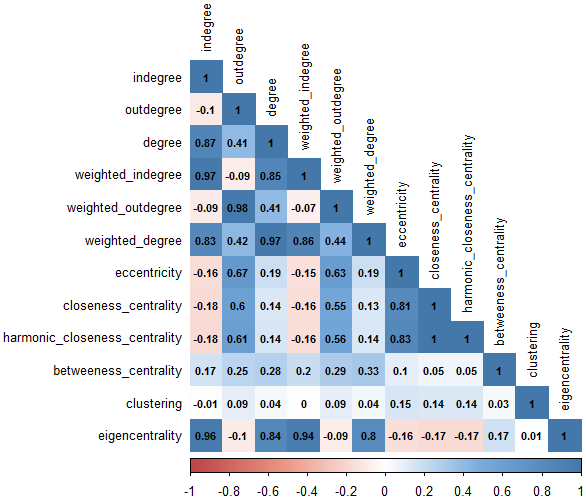
\includegraphics[width=.75\textwidth]{corr-matrix-brexit} %  % Correlation matrix
\end{figure}

\subsection{Graphs Visualization}
While mathematical metrics are essential to test hypotheses and draw sound conclusions, only a visual representation allows grasping the overall structure of a network quickly. Therefore, we show the five selected networks\footnote{Only interacting nodes are included.} in Figure \vref{network-graphs} to describe the collected data visually. These topic-network structures seem to differ on many network measures. Nevertheless, we can identify some shared features.
% Network graphs
\begin{figure}[t]
  \caption{Network graphs per topic.}\label{network-graphs}
  \begin{subfigure}[t]{.33\textwidth}
    \centering
    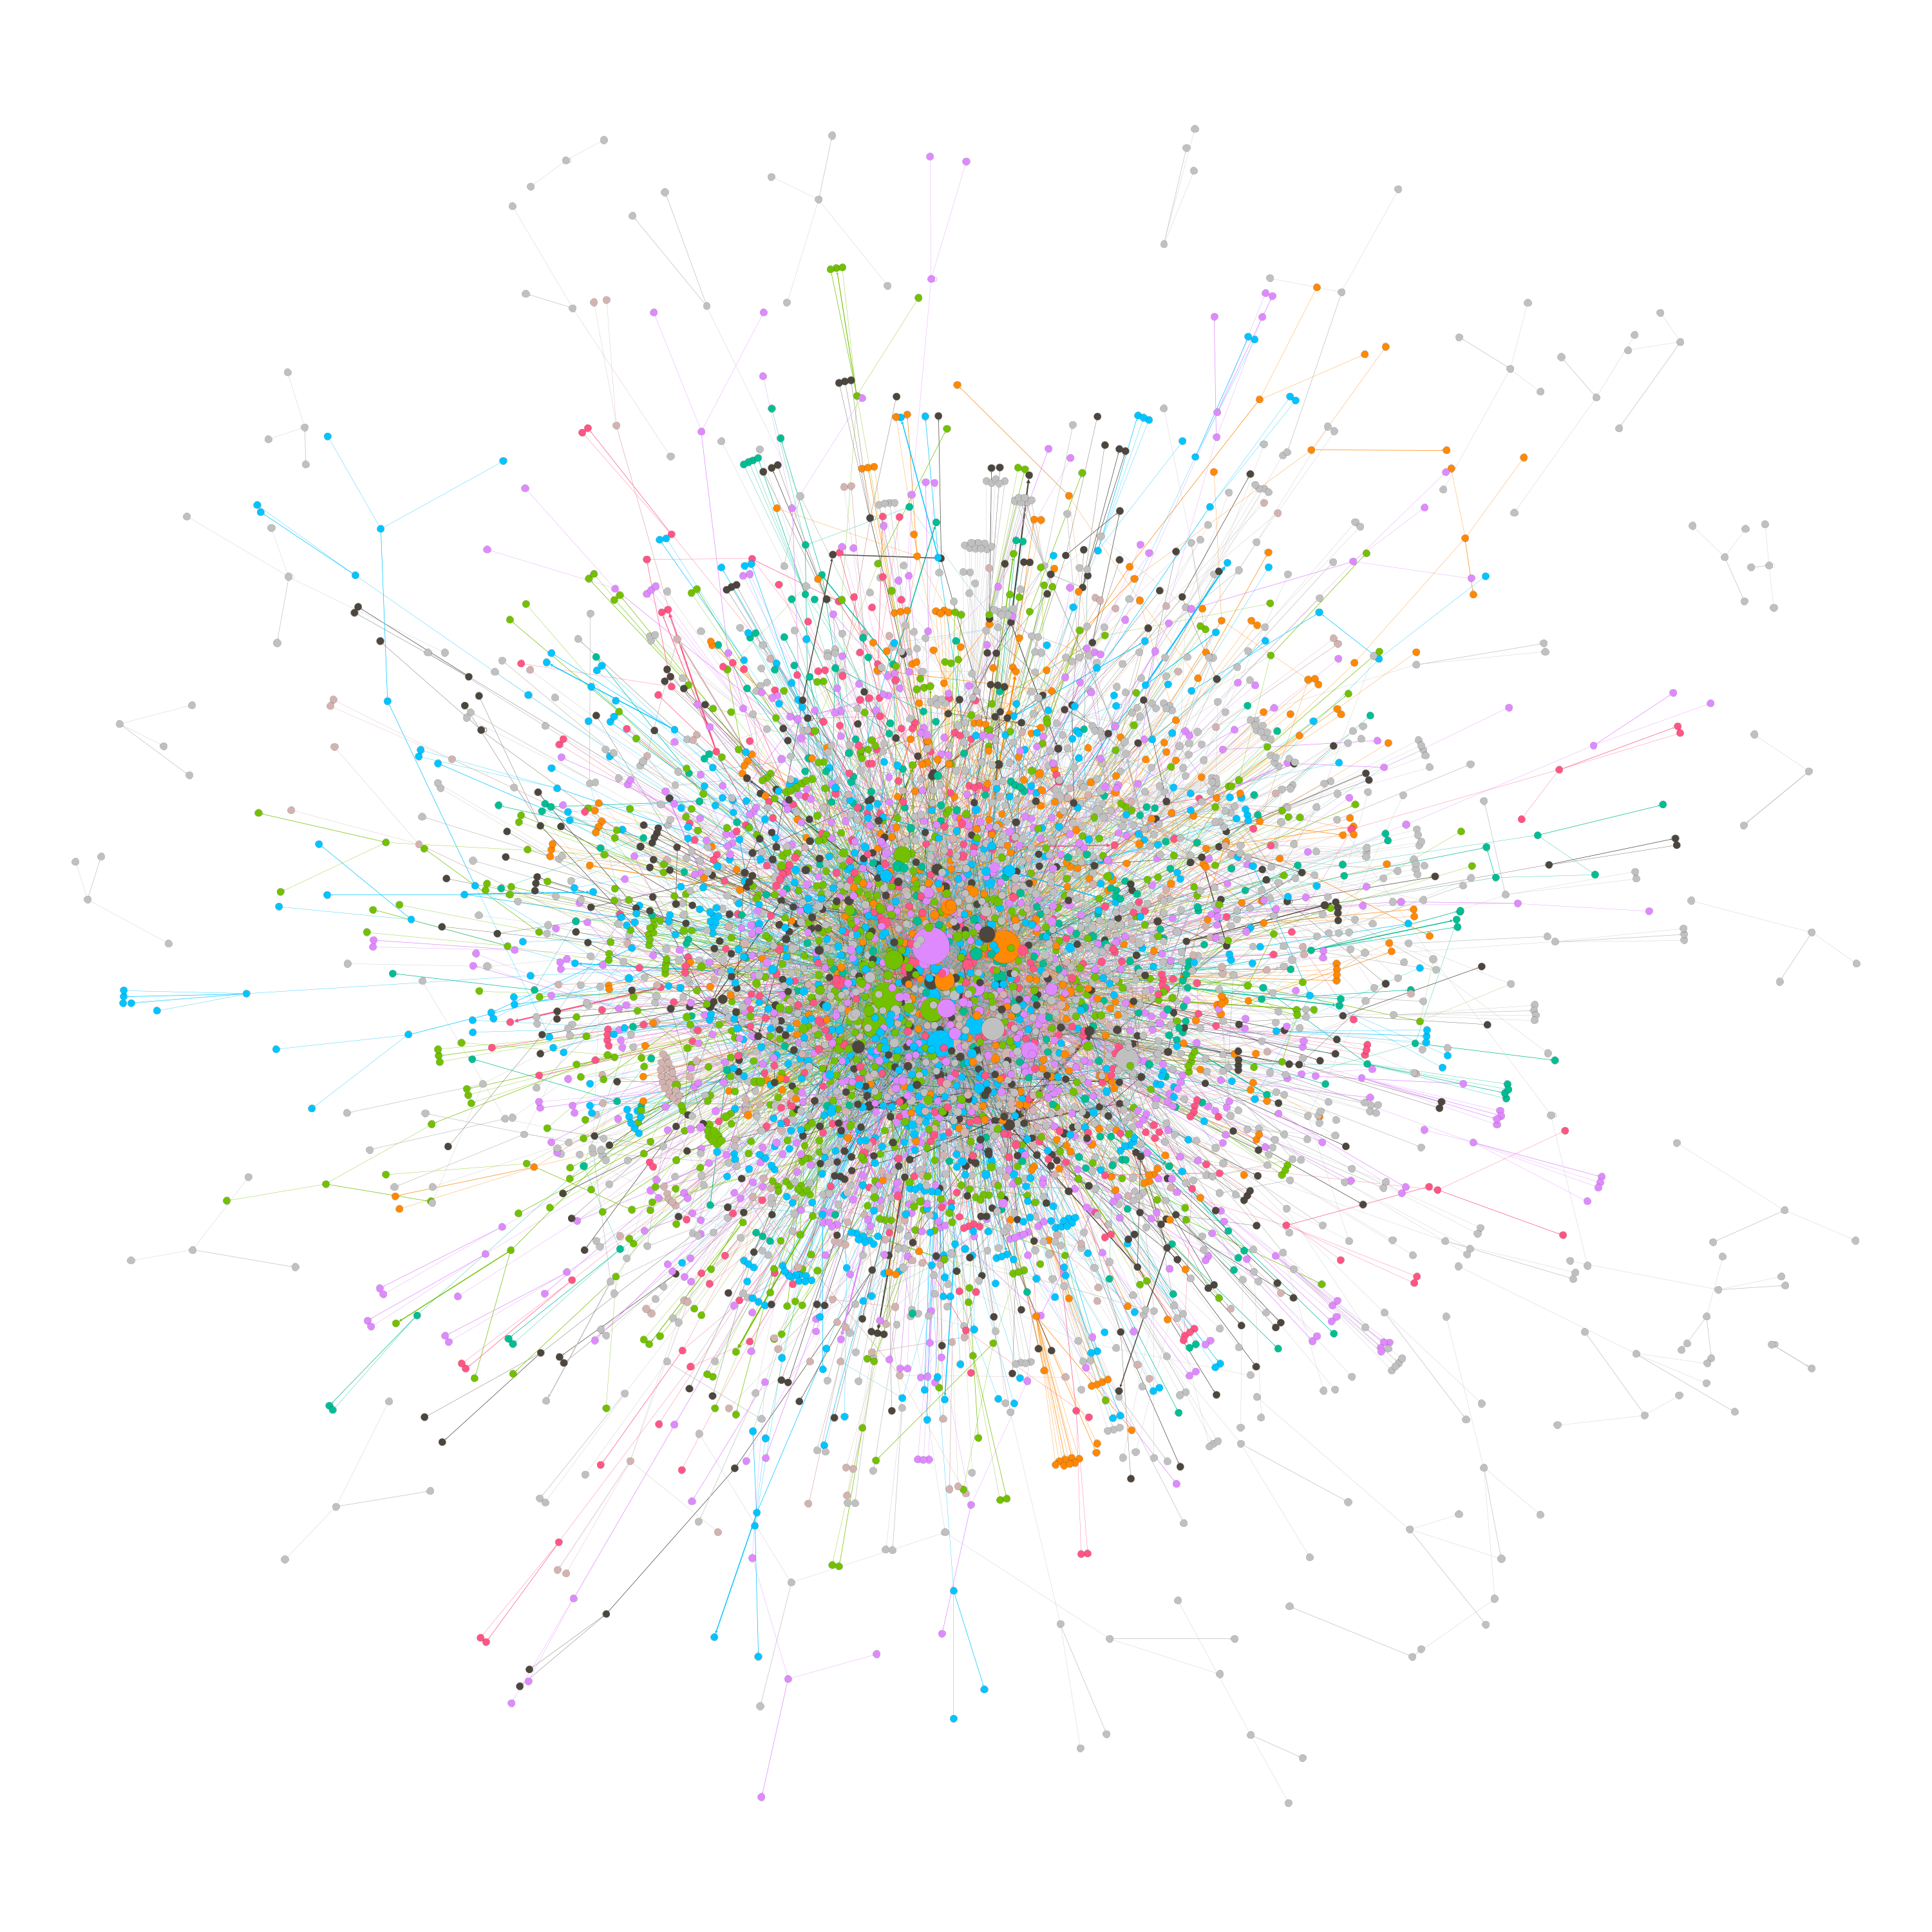
\includegraphics[width=1\linewidth]{brexit}
    \caption{Brexit}
  \end{subfigure}%
  \begin{subfigure}[t]{.33\textwidth}
    \centering
    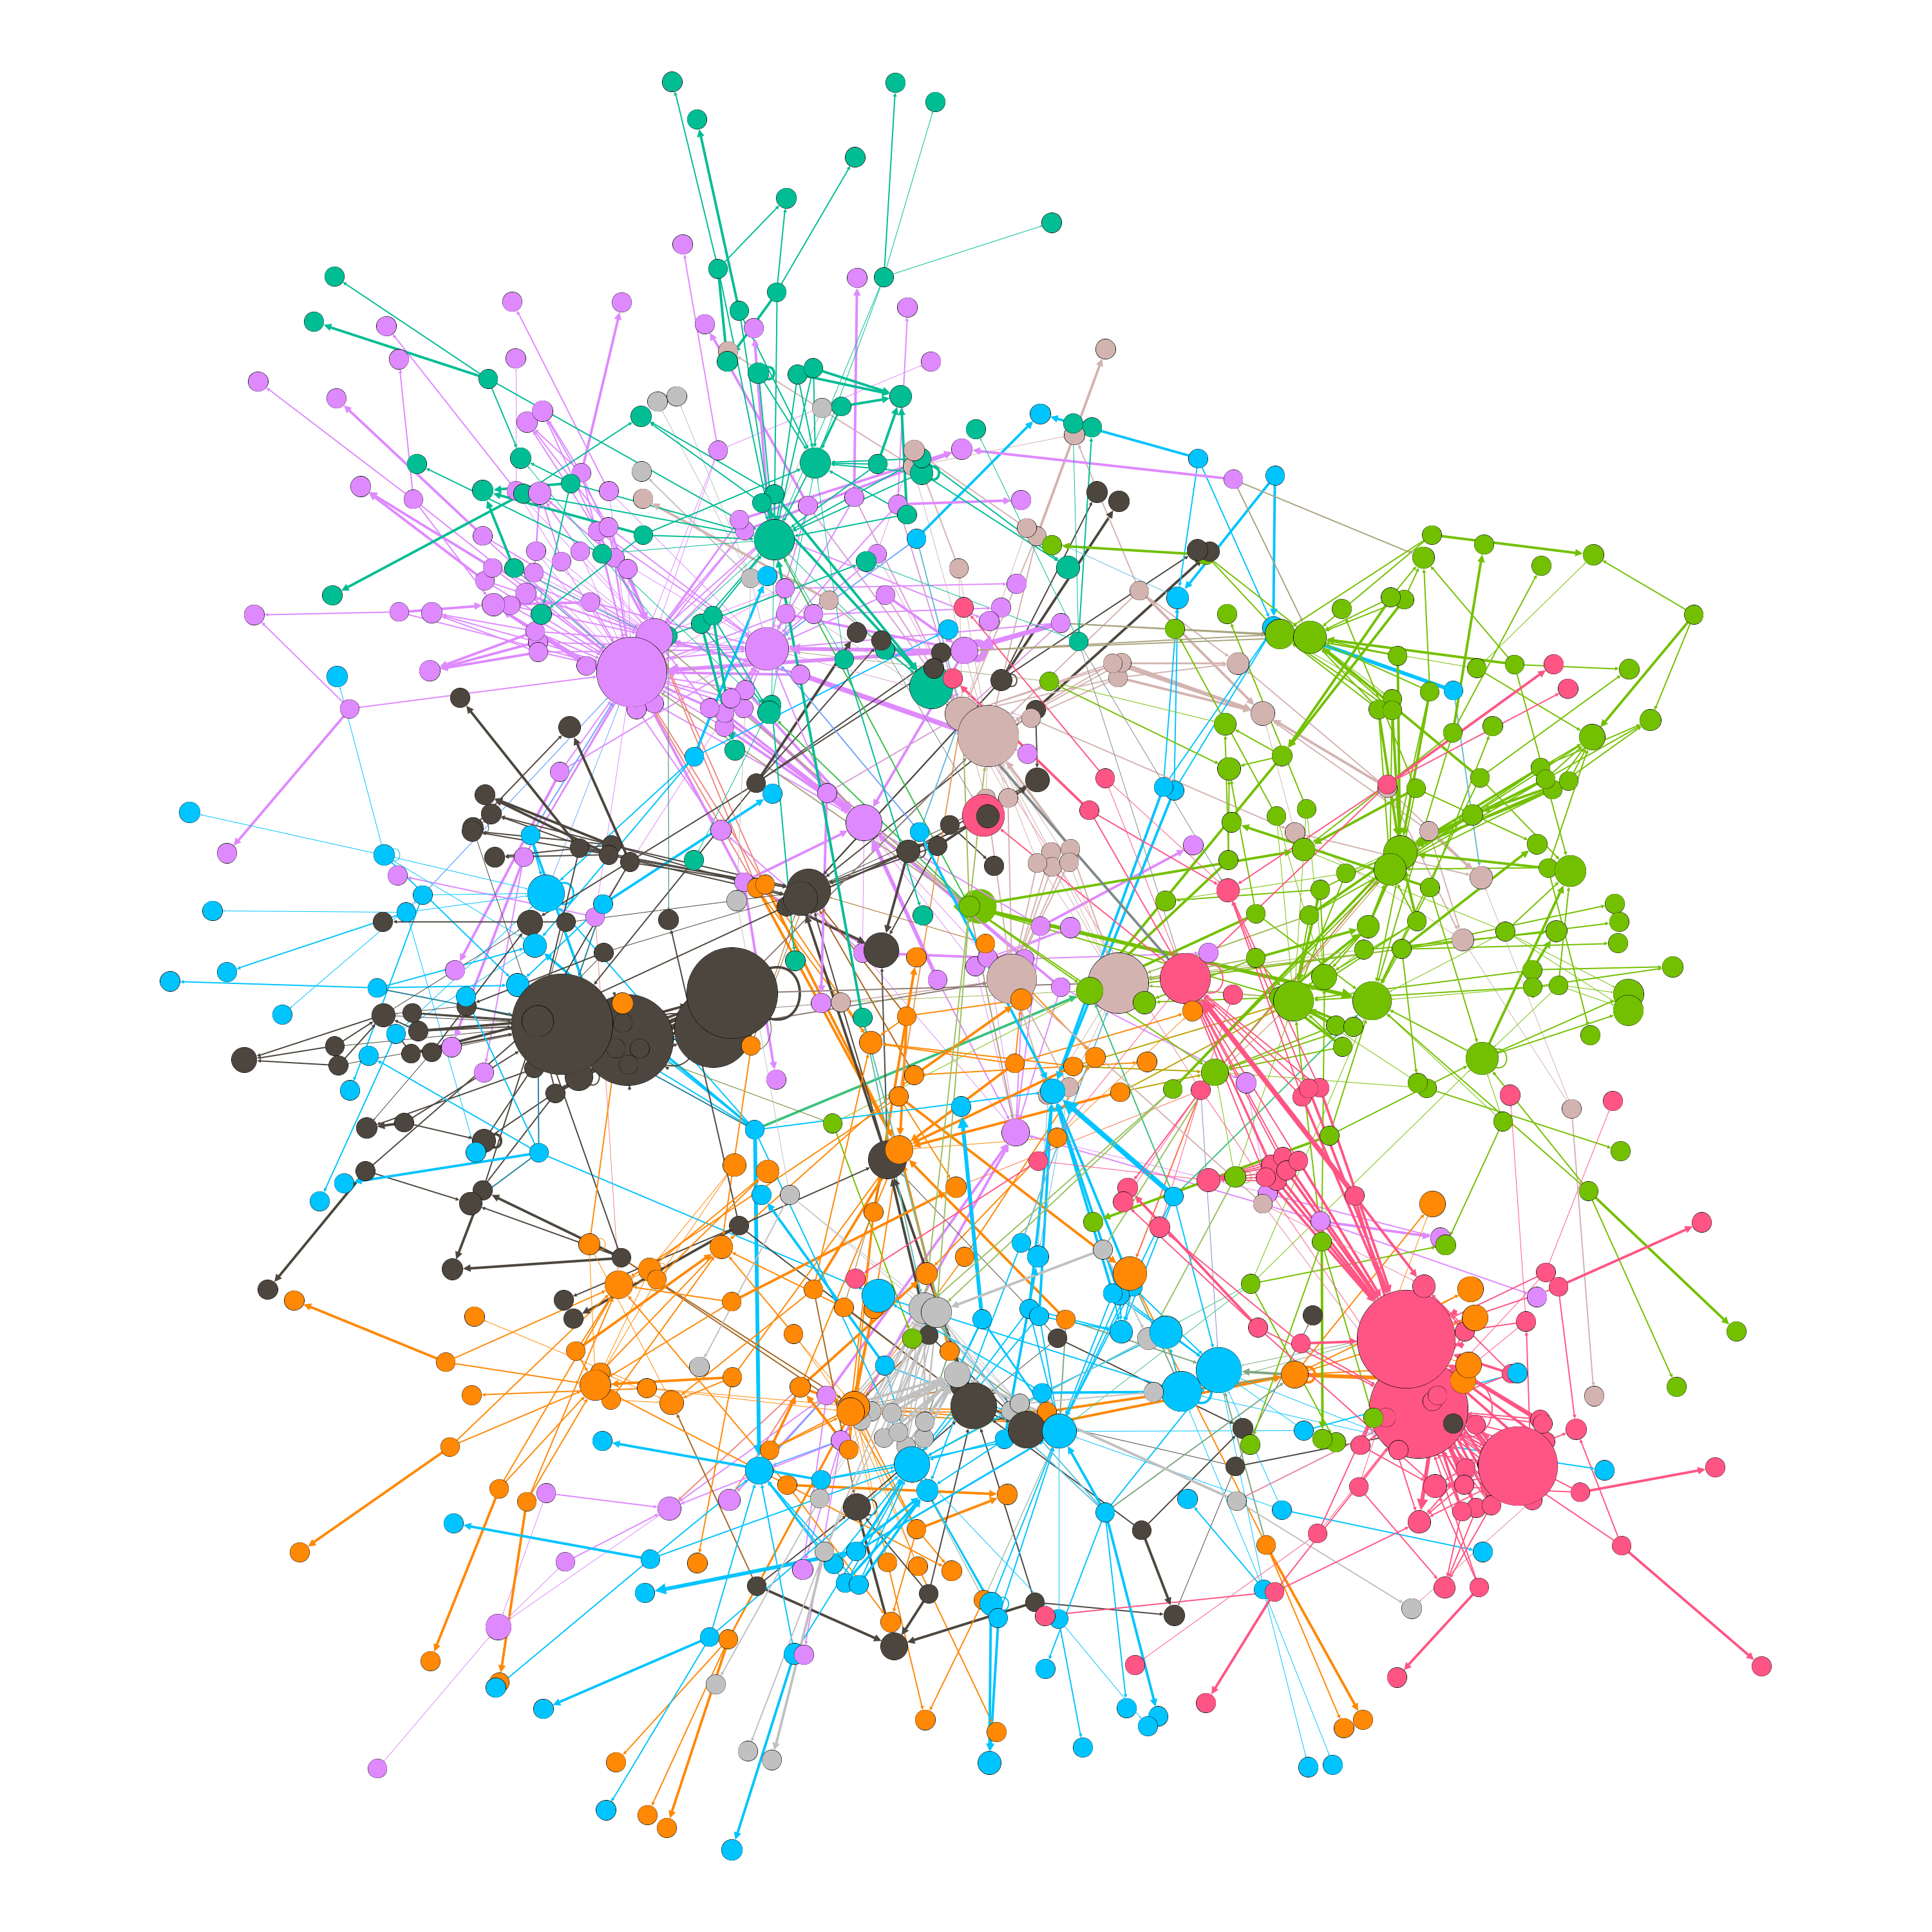
\includegraphics[width=1\linewidth]{populism}
    \caption{Populism}
  \end{subfigure}
  \begin{subfigure}[t]{.33\textwidth}
    \centering
    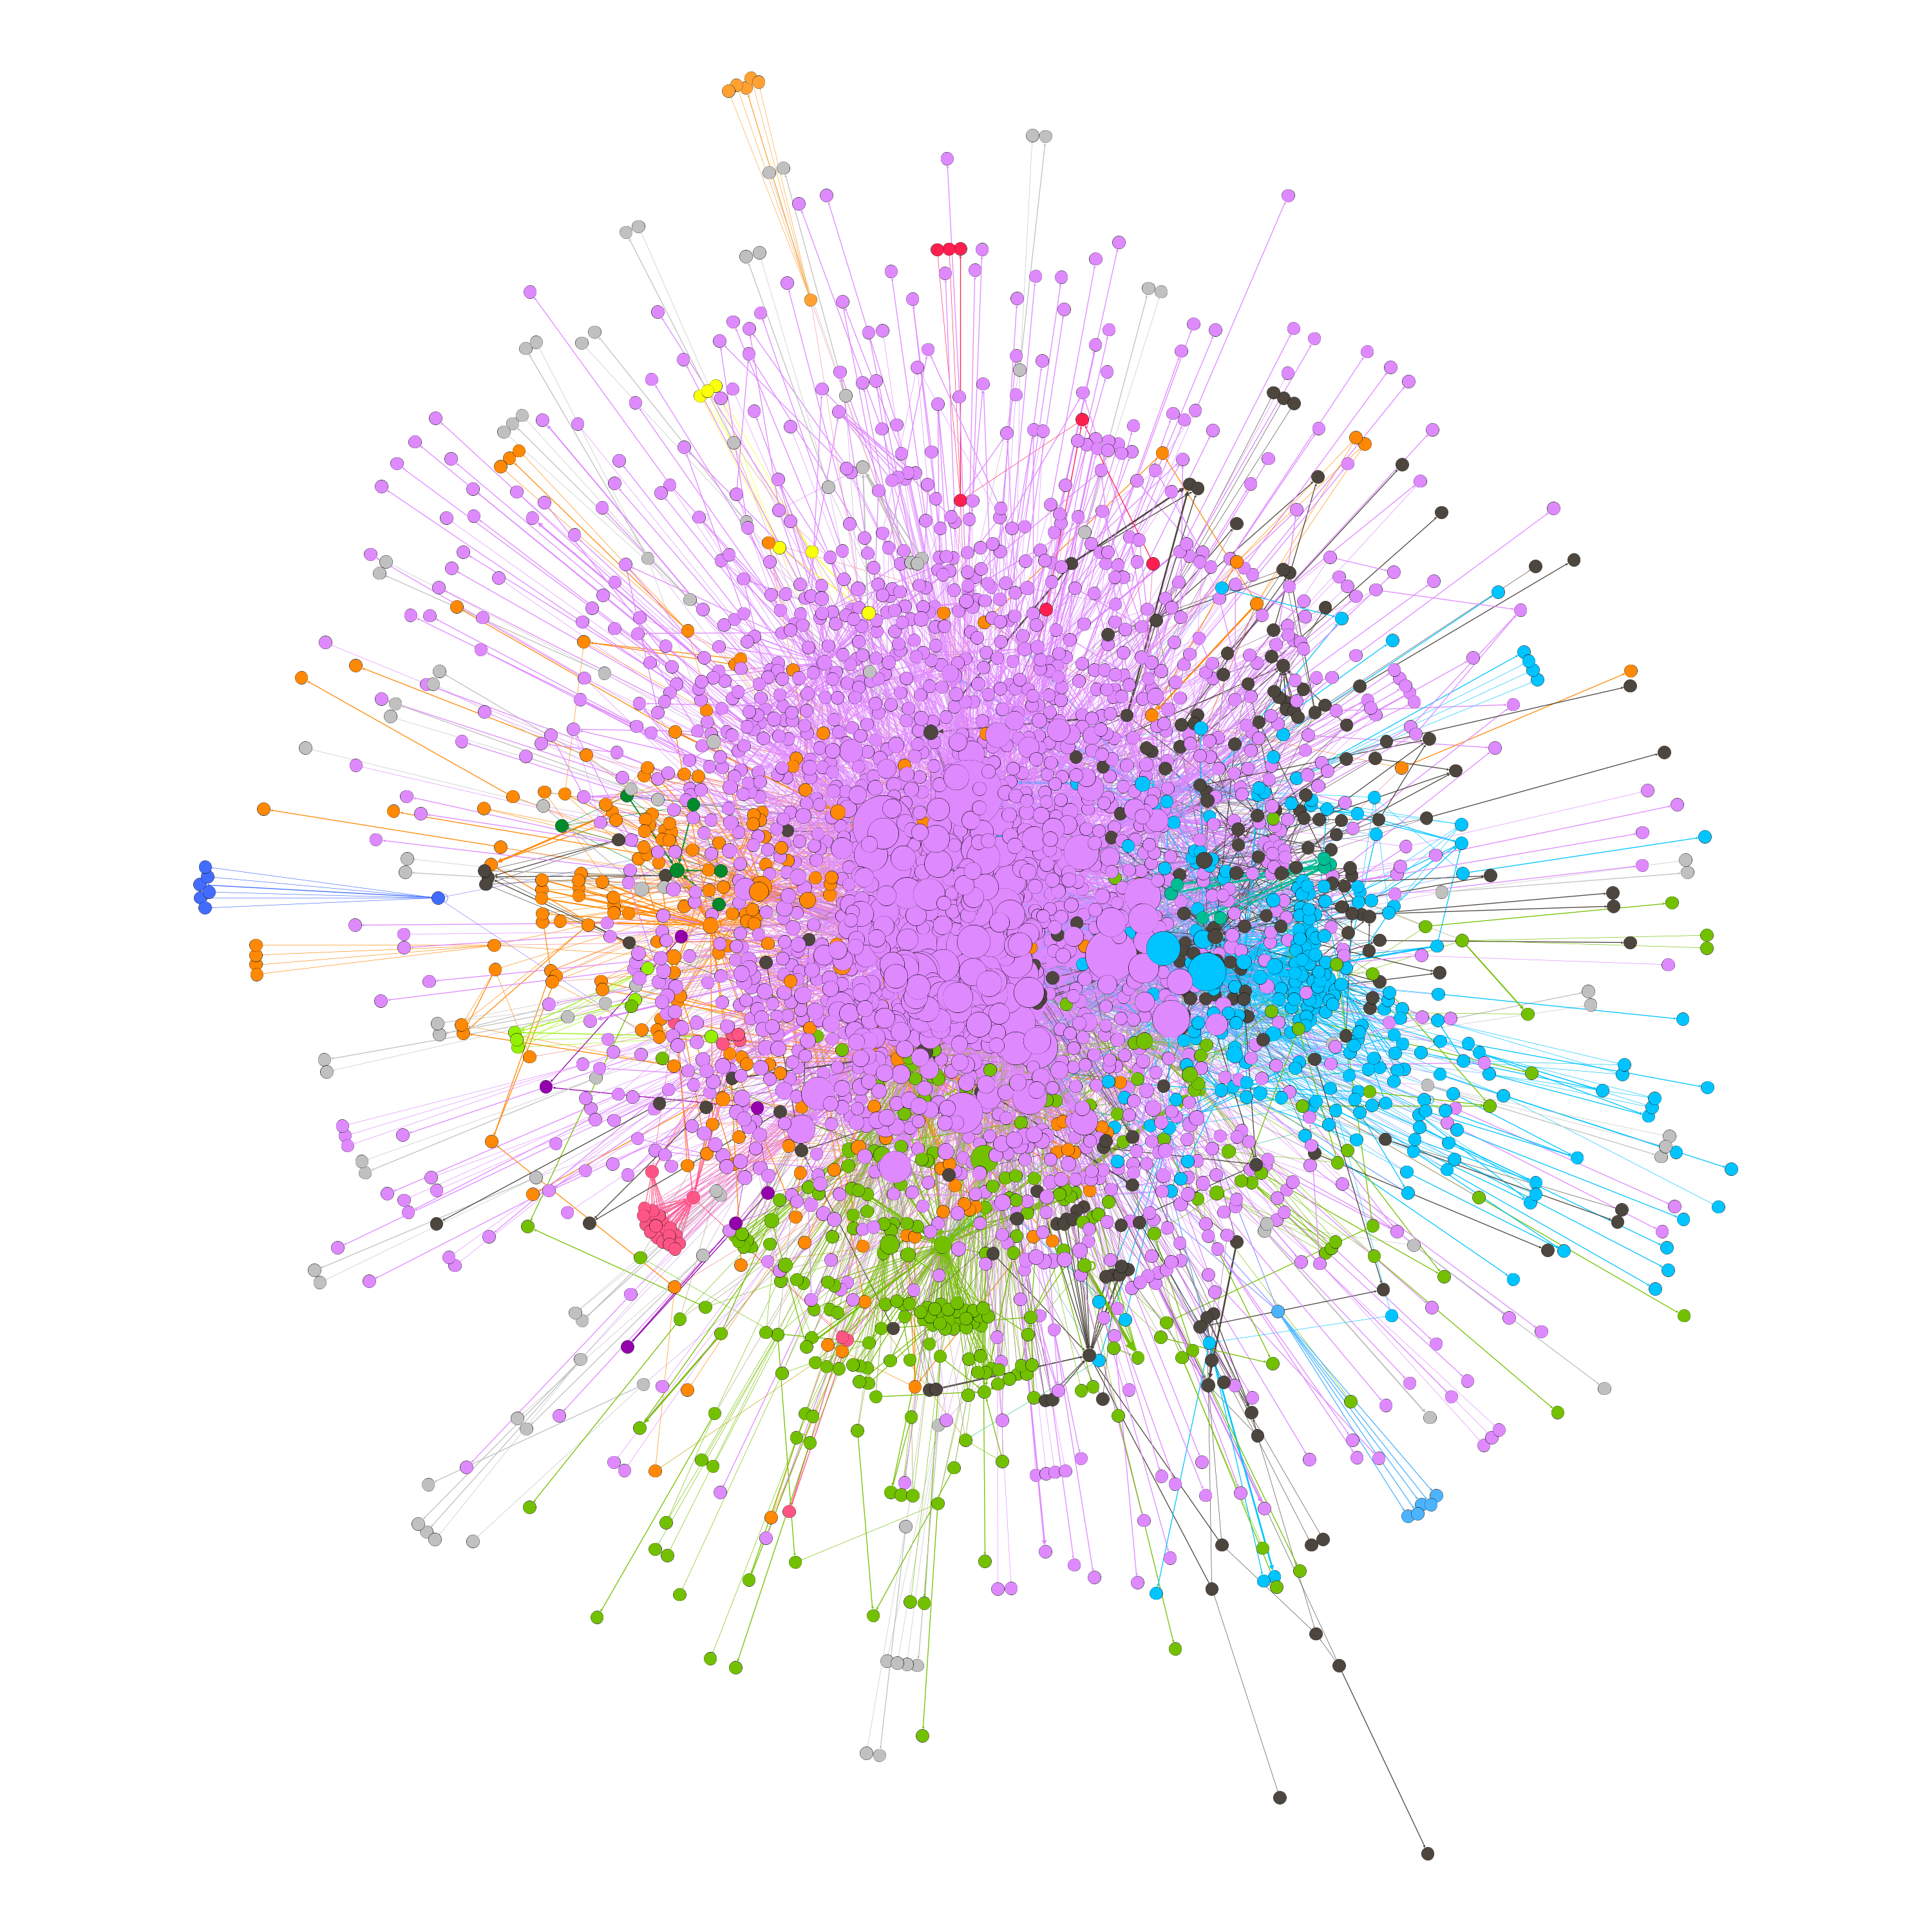
\includegraphics[width=1\linewidth]{refugees}
    \caption{Refugees}
  \end{subfigure}
  \newline
  \begin{subfigure}[t]{.5\textwidth}
    \centering
    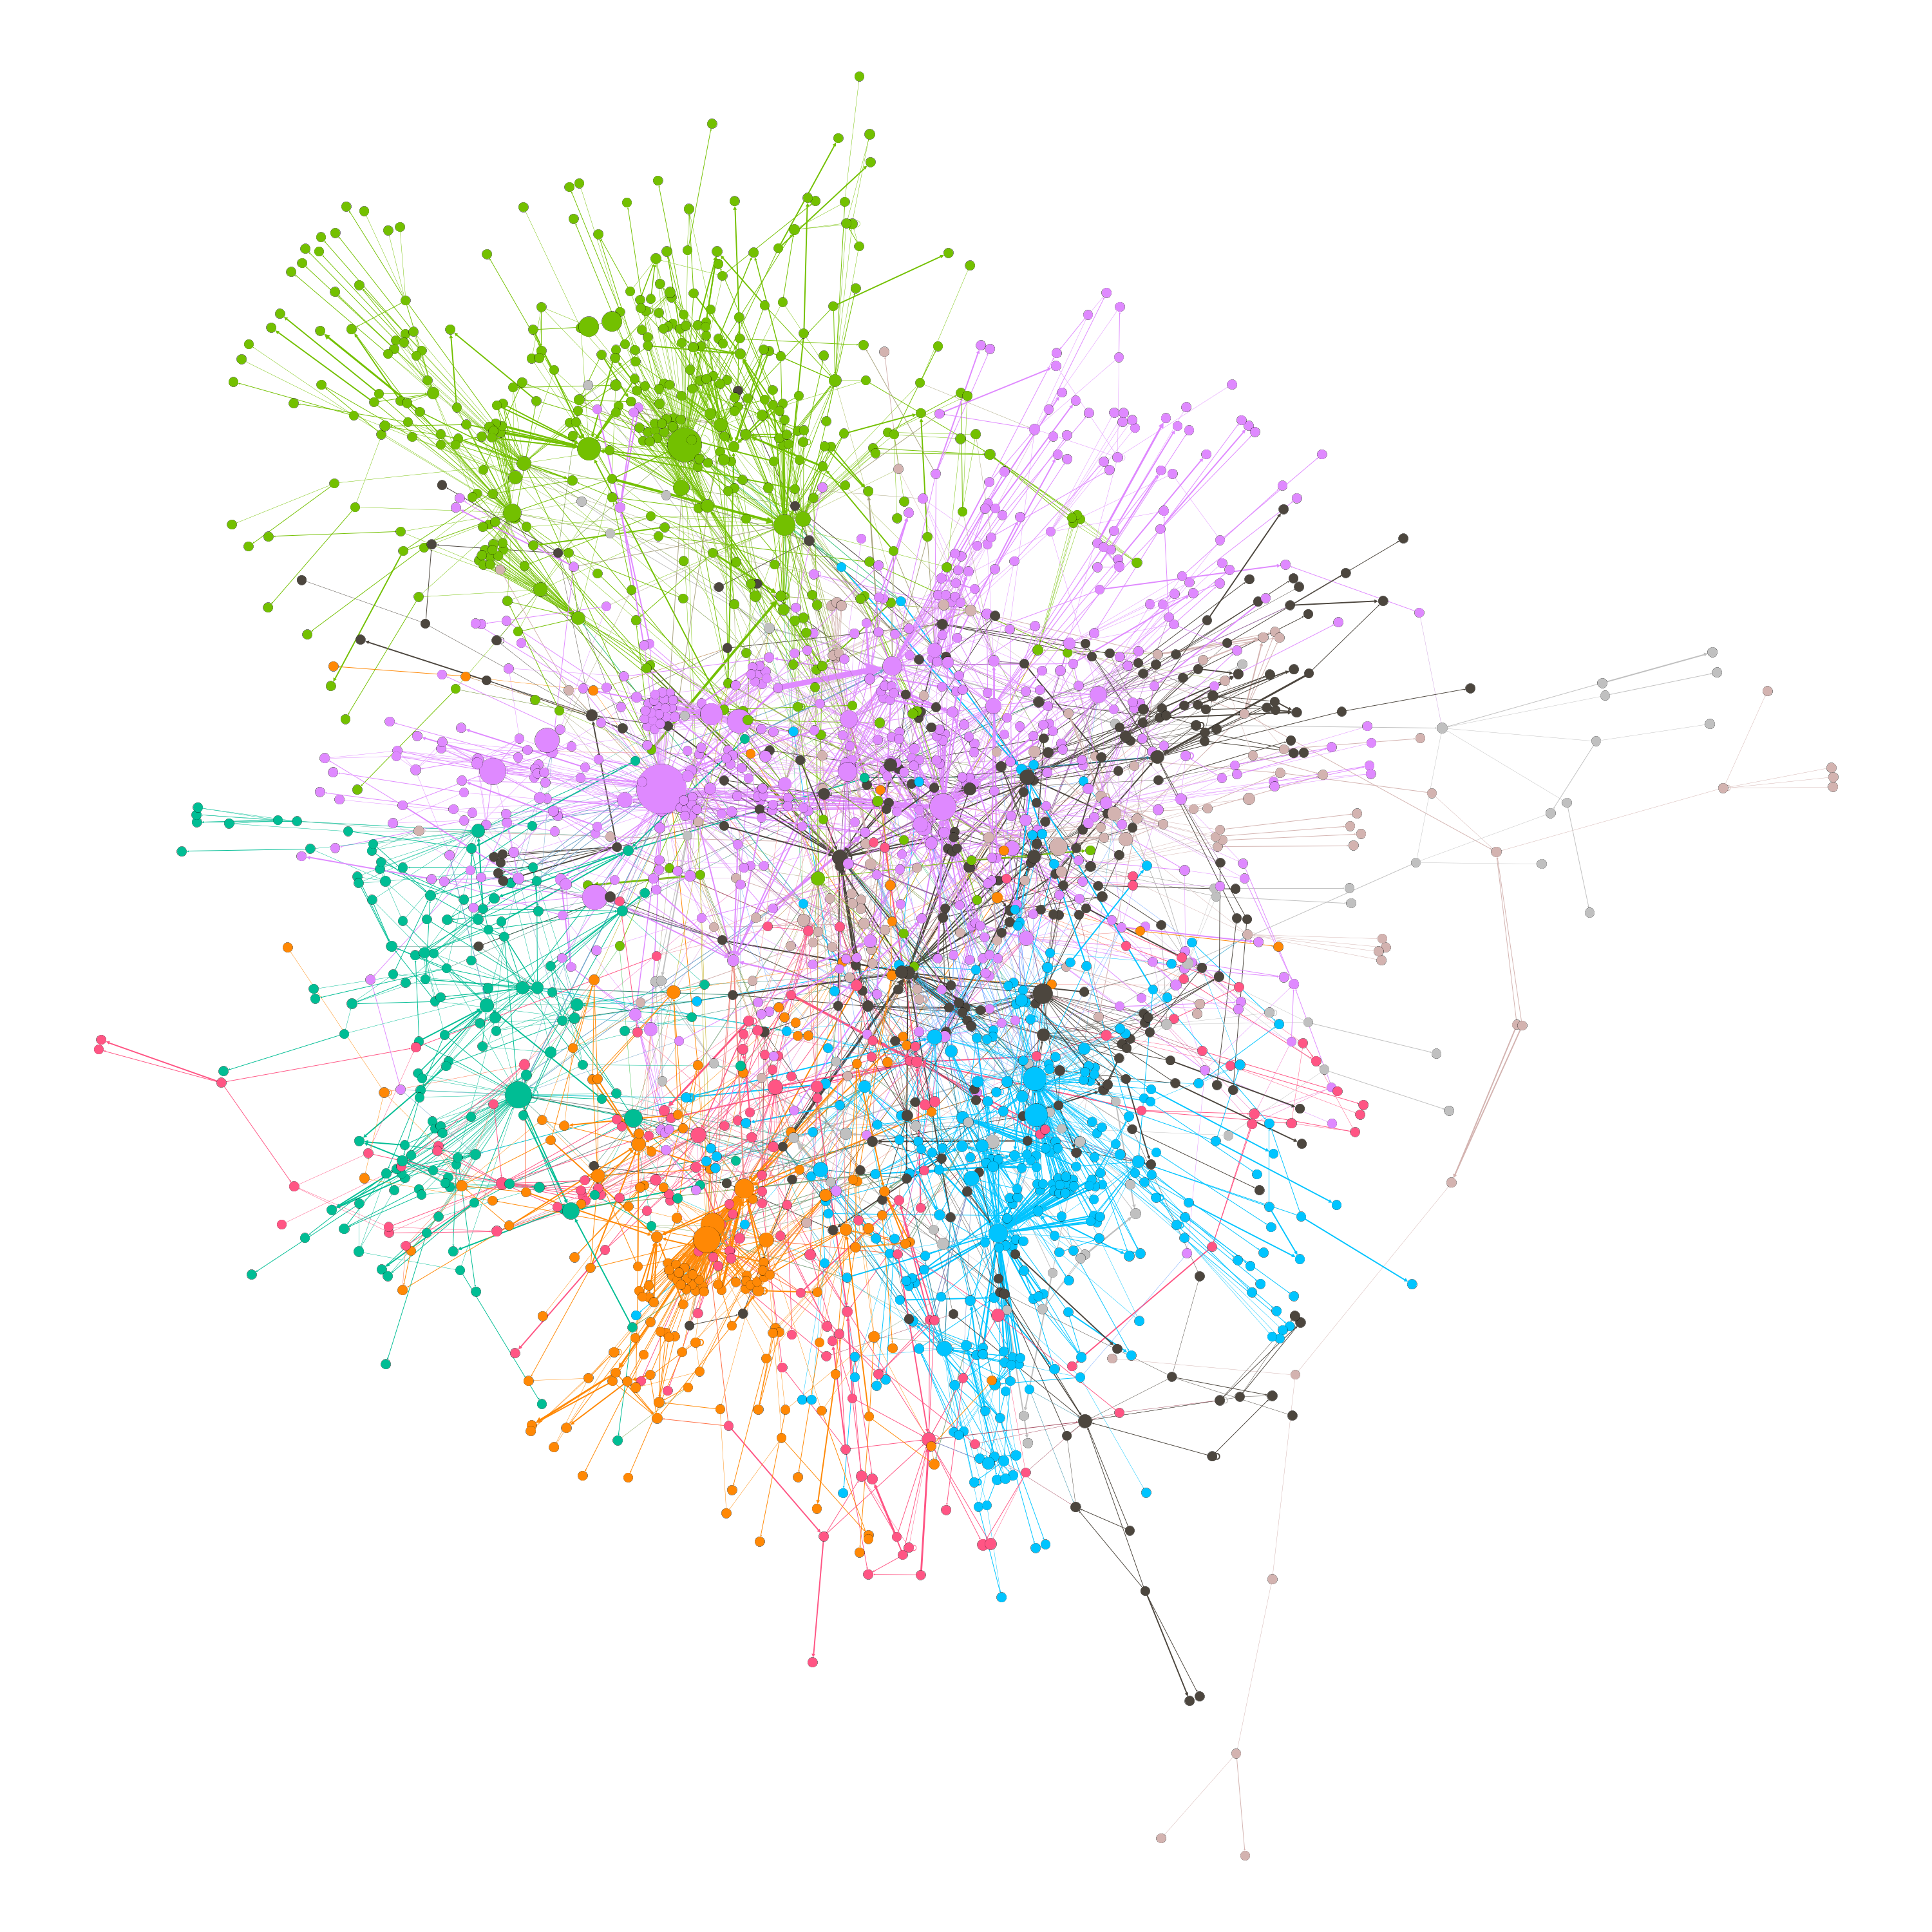
\includegraphics[width=.8\linewidth]{terrorism}
    \caption{Terrorism}
  \end{subfigure}%
  \begin{subfigure}[t]{.5\textwidth}
    \centering
    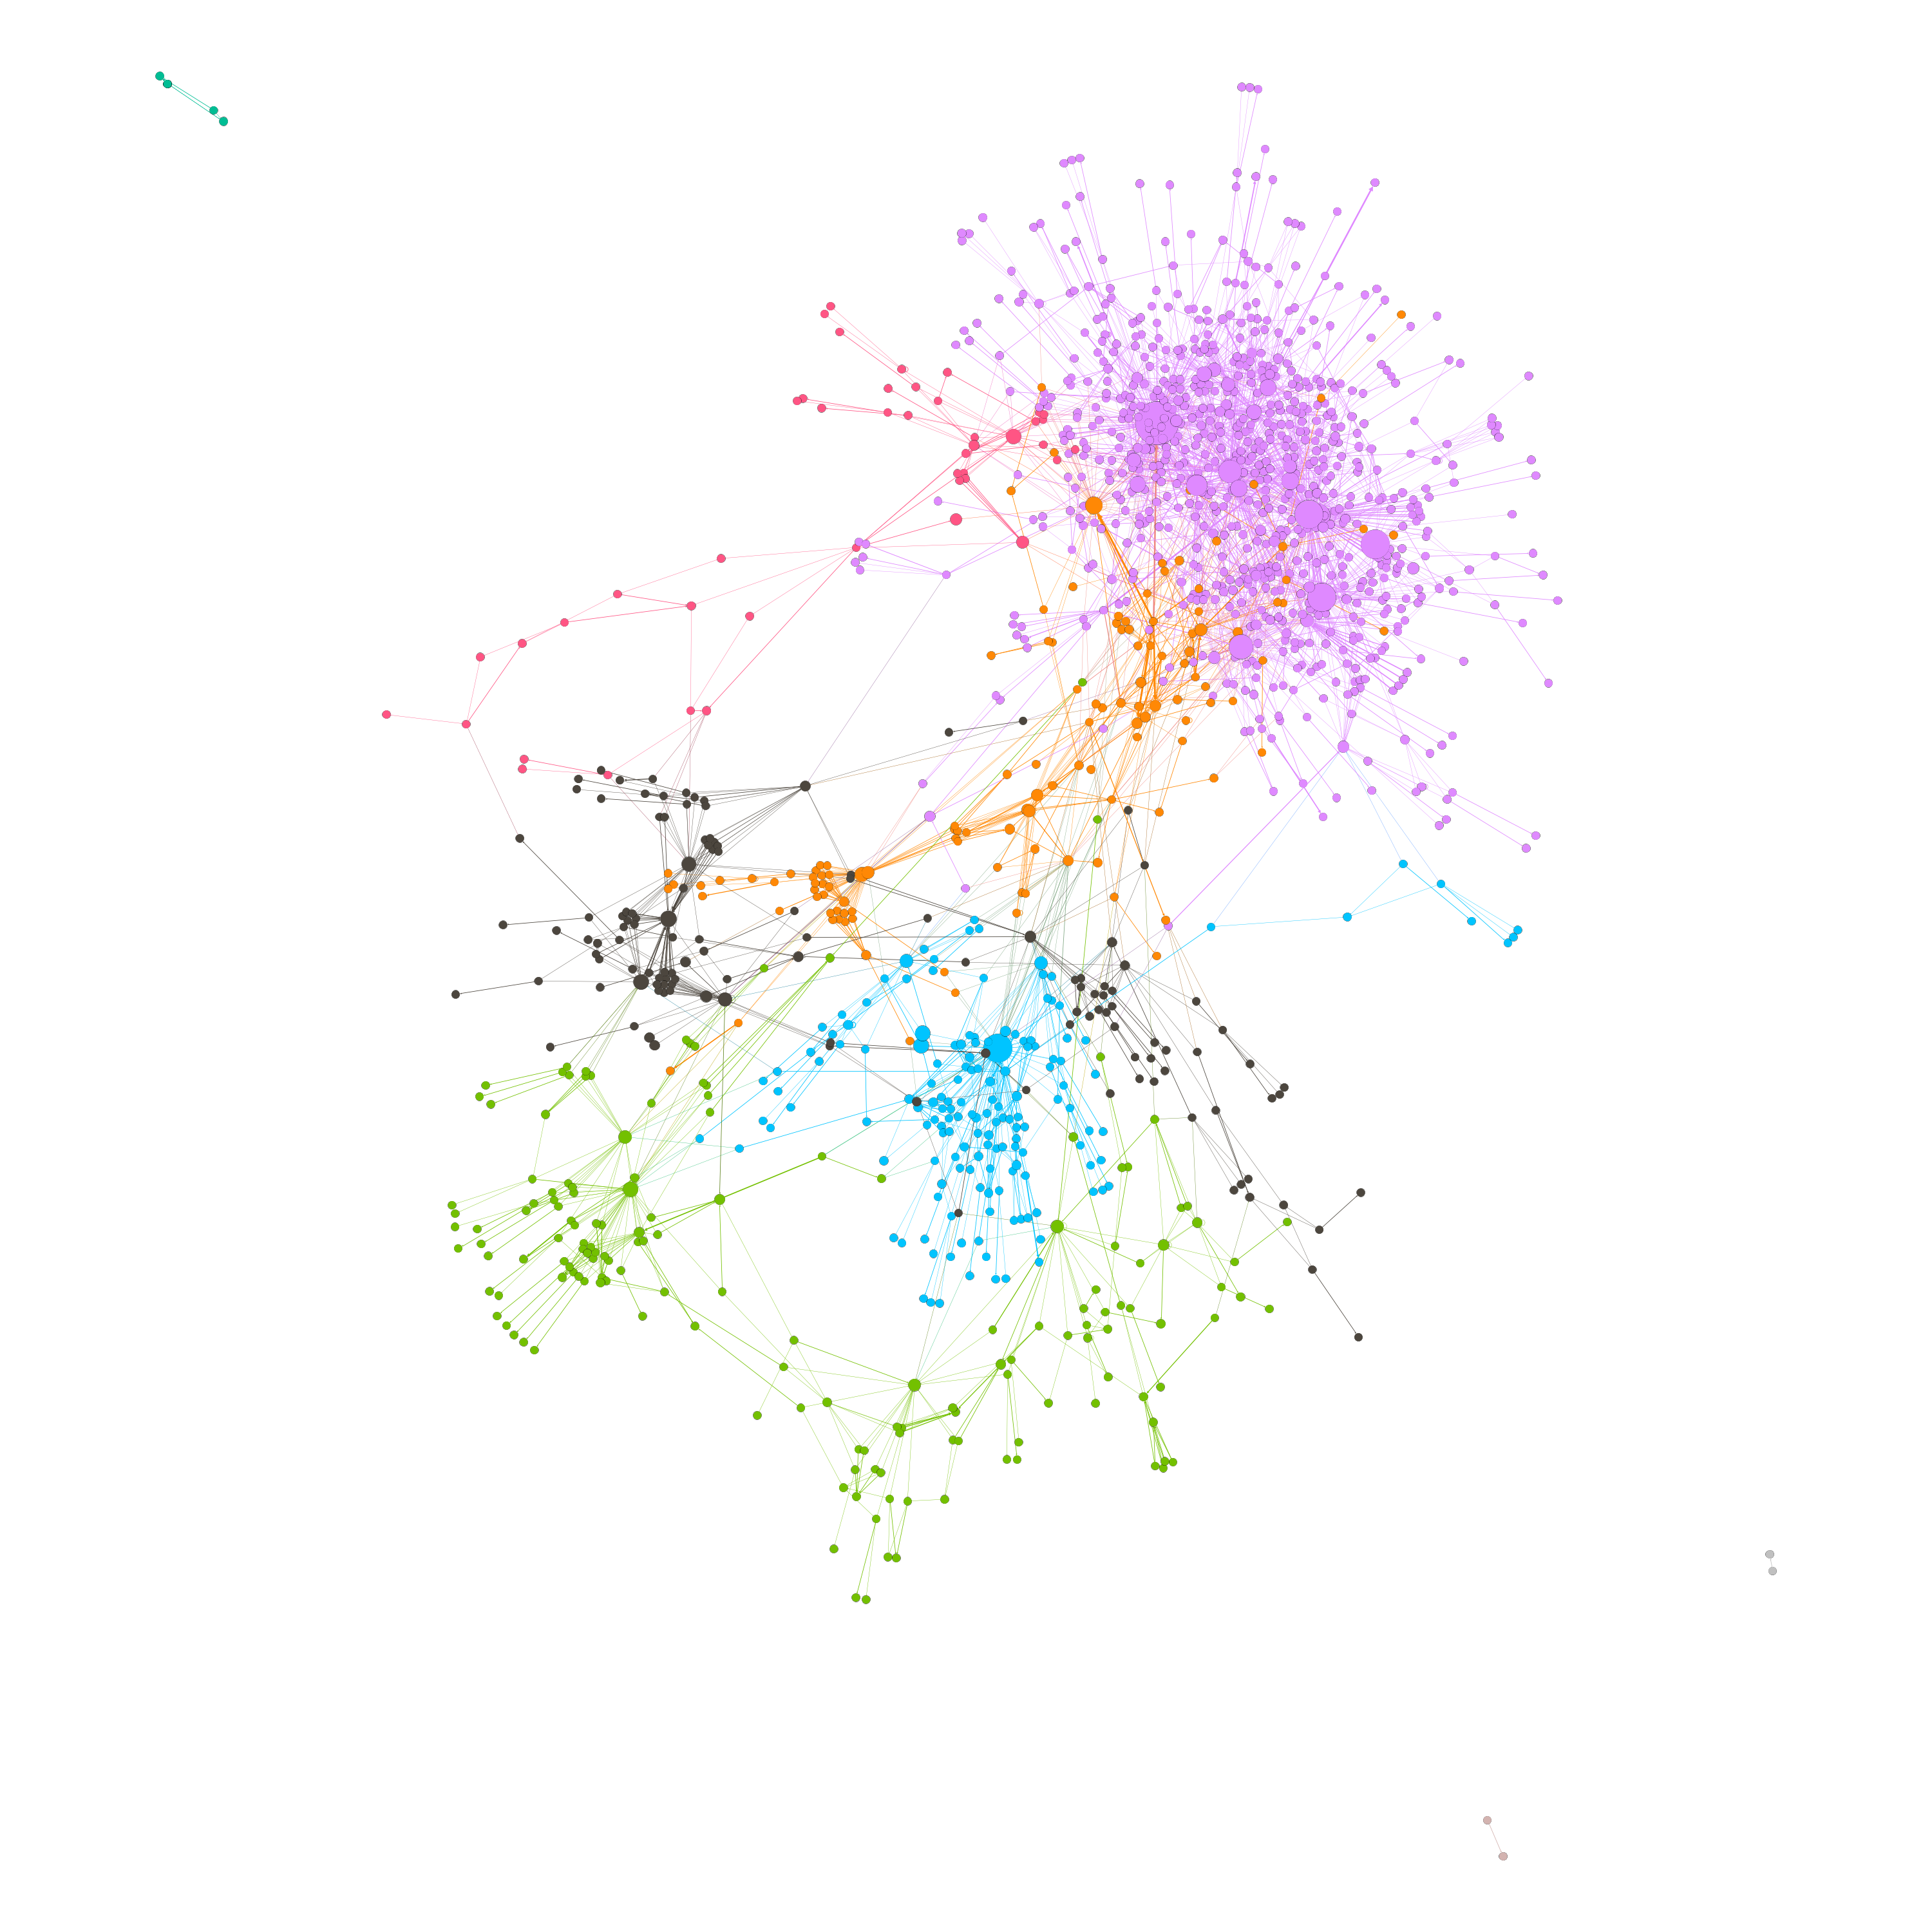
\includegraphics[width=.8\linewidth]{unemployment}
    \caption{Unemployment}
  \end{subfigure}
\end{figure}

The geographical position of nodes is determined by a force-vector algorithm\footnote{The Yifan Hu's algorithm, in our case, as mentioned earlier.} that simulates a system of physical forces: nodes tend to repulse each other, while edges hold back bounding nodes. The algorithm changes the disposition of nodes until it reaches an equilibrium where a balance of forces is guaranteed by minimizing the number of edges crossings. In other words, two nodes are closer if they are connected with each other or to the same set of nodes. Once the equilibrium is reached, the relative position of nodes reveals clusters and structural holes – the empty zone between clusters –  in the network. The color of nodes in our networks represents the community to which they belong to, determined by the modularity. Lastly, the size of the nodes represents their (eigenvector) centrality in the network.

We can classify our networks into two main groups. \texttt{Brexit} and \texttt{refugees} appear as a one, highly dense cluster, with almost no subclusters or structural holes and many sparse nodes around it. Few central individuals, called hubs, attract many connections in a star structure, where the surrounding nodes are connected to the center but not among them.

On the other hand, \texttt{populism} and \texttt{terrorism} show many small and dense subclusters, while \texttt{unemployment} has three distant and massive clusters.

\section{Models}\label{Models}\thispagestyle{SectionFirstPage} % Hide headers on the first page of the section
\subsection{Considerations on Multicollinearity}\label{multicollinearity}
Results from preliminary test models suggest severe multicollinearity issues due to the strong correlation between some variables. Because several variables in our data set measure similar concepts, we identify the most meaningful ones to include in our models.

We choose \textit{eigencentrality} among the set of available centrality measures because it takes into account the extent to which a node is connected to highly influential nodes. Furthermore, we do not include other centrality variables because they can be seen as a linear transformation of a different measure – e.g., in the case of \textit{closeness centrality} with \textit{harmonic closeness centrality} or with the proposed degree variable.

Among the group of degree measures, we select \textit{outdegree} because the number of outbound connections of a node can predict the overall number of interactions between that node and any other one in the network. Moreover, \textit{outdegree} correlates weakly with the proposed centrality measure. On the contrary, \textit{indegree} has an average positive correlation to \textit{eigencentrality} of .87 between the five topic-networks, and therefore, despite its potential contribution, we exclude it from our regressions.

We also included interaction terms in our preliminary models – between variables from different groups, and between the same variable for the source node and the target one – but all of them caused significant multicollinearity issues (VIF > 30) and did not contribute to increasing the explanatory power of the model. Thus, we decide not to include any interaction term in our final models.
\subsection{Multiple Linear Regression}
We first construct a multiple linear regression model (called model A, or complete OLS) that is run for all five topic-network structures, where the explained variable is \textit{interactions} – i.e., the number of interactions between the source and target nodes. This relationship is directed, which means that the number of interactions between nodes $A$ and $B$ might be different from the one between $B$ and $A$. We include as explanatory variables \textit{outdegree}, \textit{eigencentrality}, and the \textit{clustering coefficient} for both of the nodes in every pair of nodes (see Equation \vref{eq:1}). This model runs on all possible pairs of users in a topic-network and not only on those users who interacted with each other.

\begin{equation}
  Y=\beta_0\,+\,\beta_1\,OD_{u1}\,+\,\beta_2\,EC_{u1}\,+\,\beta_3\,CL_{u1}\,+\,\beta_4\,OD_{u2}\,+\,\beta_5\,EC_{u2}\,+\,\beta_6\,CL_{u2}+\epsilon \label{eq:1}
\end{equation}
{\footnotesize
\begingroup
\addtolength{\jot}{-5pt}
\begin{align*}
  \text{where  }~Y &= \text{number of interactions between the source and target nodes (directed)} \\
  OD\textsubscript{u1} &= \text{outdegree for the source node} \\
  EC\textsubscript{u1} &= \text{eigencentrality for the source node} \\
  CL\textsubscript{u1} &= \text{clustering for the source node} \\
  OD\textsubscript{u2} &= \text{outdegree for the target node} \\
  EC\textsubscript{u2} &= \text{eigencentrality for the target node} \\
  CL\textsubscript{u2} &= \text{clustering for the target node}
\end{align*}
\endgroup
}%
\subsection{Logistic and Conditional Linear Regression}
We build a logistic regression model (model B, or logistic) to predict the likelihood that paired users will interact with each other. Therefore, the dependent variable is the dichotomous \textit{interacted}. The independent variables are the same as in model A (see Equation \vref{eq:2}).

\begin{equation}
  P(interacted)=\frac{e^{b_0\,+\,b_1\,OD_{u1}\,+\,b_2\,EC_{u1}\,+\,b_3\,CL_{u1}\,+\,b_4\,OD_{u2}\,+\,b_5\,EC_{u2}\,+\,b_6\,CL_{u2}}}{1+e^{b_0\,+\,b_1\,OD_{u1}\,+\,b_2\,EC_{u1}\,+\,b_3\,CL_{u1}\,+\,b_4\,OD_{u2}\,+\,b_5\,EC_{u2}\,+\,b_6\,CL_{u2}}} \label{eq:2}
\end{equation}

\vspace{15pt}
Finally, we build another multiple linear regression model (model C, or conditional OLS), which runs on a filtered subset of our data for all the pairs of nodes where \textit{interacted} is true (1). The model equation is the same as Equation \vref{eq:1}.

\section{Results}\label{Results}\thispagestyle{SectionFirstPage} % Hide headers on the first page of the section
Table \vref{model-a} displays the results from the multiple linear regression models (A) for each topic. F test is significant at 1\% in all topic-networks and, unless otherwise noted, all coefficients are statistically significant at the 0.01 level too. We detect no issues of multicollinearity  – VIF is never higher than 1.24 – but R\textsuperscript{2} is extremely low. However, model fit is not a priority in the context of this research because we do not aim for an accurate prediction, but rather to assess whether a (perhaps small) reliable relationship exists among the considered variables. Even though the models do not explain much of the variation of the data, they are still significant. Indeed, trying to predict the number of interactions between two users exclusively based on their network characteristics is an unhelpful oversimplification of reality. Outcomes could be dictated by many latent factors at play that may affect other facets of the model.

The $EC_{u2}$ predictor is the most potent one in explaining the dependent variable in models A. It seems that users are more likely to have interacted with highly influential (central) users, holding all other regressors constant. However, the magnitude of coefficients is generally very modest among these models. We suspect that this is because the effects of the vast majority of nodes that did not interact (N = 23,440,660 in the case of \texttt{brexit}) considerably mitigate those of the relatively rare nodes that did it (N = 9,146). In pursuit of more extreme coefficients, we take into account whether two nodes interacted and therefore build models B and C.

Table \vref{model-b-c} shows the outcomes of models B and C for each topic-network.
All five logistic regressions (models B) fit the data well since the Nagelkerke's R\textsuperscript{2} is generally close to 20\%. We find no significant multicollinearity issues, and VIF scores never higher than 1.30, except for $OD_{u1}$ (VIF = 6.74) and $EC_{u1}$ (VIF = 6.52) in the \texttt{refugees} model but we deem these values acceptable. All coefficients are statistically significant at 1\%, except for those of $CL_{u2}$, and the magnitude of effects is generally stronger than in the previous models.

In the \texttt{brexit} case, $EC_{u1}$ is the regressor with the strongest partial effect on the explained variable. However, it is a rather powerful predictor in the other four models too. Thus, it seems that more central users are less likely to have initiated a conversation or replied to one compared to less central users, ceteris paribus. On the other hand, $EC_{u2}$ coefficients are positive and significant at 1\%, suggesting that users are more likely to have interacted with central users rather than with less influential ones.

The positive and significant coefficients of $OD_{u1}$ follow the intuitive concept that a higher number of outbound messages from the source user increases the probability of interaction between that user and any other one in the network. On the contrary, $OD_{u2}$ estimates are generally negative and significant at 1\%. Overall, our data reveal that the target node's coefficients are of opposite sign than those of the source node in all models B.

Lastly, the coefficients of $CL_{u1}$ are positive and significant at the 0.01 level as well, indicating that, all else being equal, more clustered nodes are more likely to have interacted with other nodes. Instead, $CL_{u2}$ is not significant, except for \texttt{refugees} and \texttt{unemployment}, where it shows a positive relationship with the outcome measure.

Results from models A and B indicate that node-level network characteristics may not differ between distinct topics of discussion. However, we cannot conclude this without first interpreting results from models C.

The last multiple linear regression models (C) are run on a filtered subset of our data, for all the pairs of nodes where the number of interactions is above zero. Hence, we can juxtapose the results of models C to those of models B, gaining an insight into the mechanism underlying the number of interactions between users, given that they have interacted.

The F statistic is significant at 1\% for all topic-networks in models C except for \texttt{populism}, for which it is significant at 10\%. R\textsuperscript{2} is still low compared to models A, but it improves substantially for the topic \texttt{refugees} (R\textsuperscript{2} = .201). The coefficients in these models fluctuate considerably between distinct topic-networks, and therefore it is more challenging to find a shared pattern of relationships. To compare the magnitude of effects between different topic-network structures and models for the same variable, we need to test the significance of the coefficients' differences pairwise. Because this task is painfully impractical due to the number of variables, models, and groups involved, we graph the models' coefficients and their standard errors (with a 95\% confidence interval) to compare estimates visually.

\begin{figure}
\caption{Coefficients and SE per topic for $EC_{u1}$ and $EC_{u2}$.}\label{eigenxu2eigencoeff}
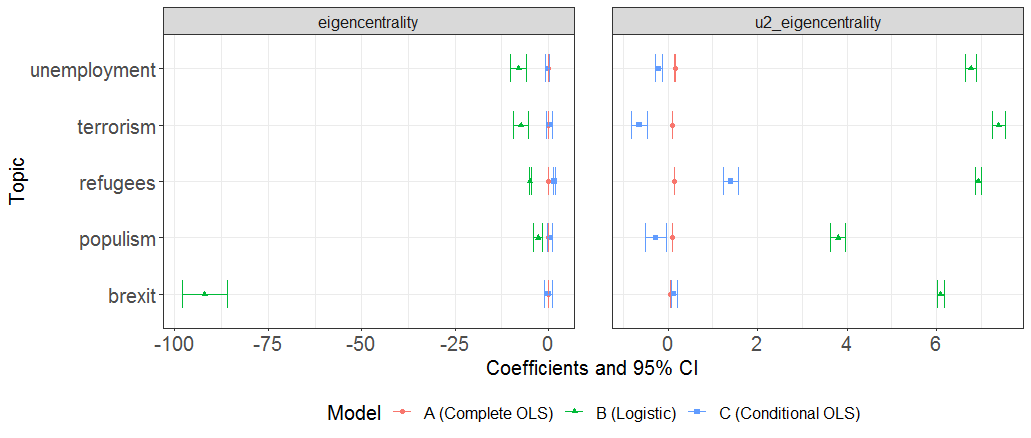
\includegraphics[width=\textwidth]{eigenxu2_eigen}
\caption*{\footnotesize$EC_{u1}$: We observe that the magnitude of effects varies between topic-networks in models B.\\$EC_{u2}$: We observe that the sign of the relationship varies between topic-networks in models C.}
\end{figure}

Figure \vref{eigenxu2eigencoeff} shows these graphs for $EC_{u1}$ and $EC_{u2}$. For instance, we observe that most of the $EC_{u2}$ coefficients' standard errors and their confidence intervals do not overlap (this is particularly evident in models B and C). When the error bars do not overlap, the difference between models' estimates may be significant\footnote{A statistical test should be performed to draw a conclusion.}. On the contrary, if error bars do overlap, we can conclude that the difference is not significant, and therefore that the paired coefficients do not statistically differ from each other. Thus, we infer that the $EC_{u2}$'s coefficients may statistically differ, and we speculate that this might be due to the intrinsic characteristics of the respective topic-network structures. In other words, structures with unique network characteristics – in terms of degree, centrality, and clustering – exist for different topics of discussion.
Similar graphs to Figure \ref{eigenxu2eigencoeff} for all variables can be found in the Appendix \vrefrange{model-a-coeff}{model-c-coeff}.

In summary, we find that the \textit{eigencentrality} of the target node ($EC_{u2}$) positively predicts the interaction and the number of interactions between nodes, regardless of the discussion topic. However, among those pairs of nodes that interacted, the direction of the effect of this variable on the number of interactions varies between topics. By contrast, the \textit{eigencentrality} of the source node ($EC_{u1}$) negatively influences the probability of interaction, but not the extent to which pairs of users interact with each other. Therefore, we conclude that the effect of \textit{eigencentrality} varies on whether it refers to the source or target node.

As regards the source's \textit{outdegree} ($OD_{u1}$), our data indicate that this positively influences both the probability of interactions and the number of interactions, regardless of the topic in discussion. However, given that two nodes have interacted, the direction of the effect of $OD_{u1}$ fluctuates between topics, although in a weaker way than the one of $EC_{u2}$. On the other hand, the target's \textit{outdegree} ($OD_{u2}$) negatively affects the probability of interaction between two nodes, regardless of the topic (except for \texttt{refugees}). However, among those pairs of users who interacted, the effect is overturned (positive and significant) for all topic-network structures.

Finally, we find that, regardless of the topic, both a highly clustered neighborhood of the source and target nodes ($CL_{u1}$ and $CL_{u2}$) positively influence the probability of interaction. Nevertheless, given that two nodes have interacted, highly dense clusters negatively affect the number of interactions between nodes (this is especially evident for \texttt{refugees}).

\clearpage % Multilm output table
\thispagestyle{SectionFirstPage}
\renewcommand{\arraystretch}{1.35}
\begin{sidewaystable}[!htbp]
  \centering
  \caption{Regression models A (Complete OLS) per topic.}
  \label{model-a}
  % Set table width
  \resizebox{0.7\width}{!}{\begin{tabular}{@{\extracolsep{0pt}}lccccc}
  \hline
   & \multicolumn{5}{c}{\textit{Dependent variable:}} \\
   \cline{2-6}
   \\[-2.8ex] & no. of interactions & no. of interactions & no. of interactions & no. of interactions & no. of interactions \\
   \\[-2.8ex] & (1) & (2) & (3) & (4) & (5)\\[+1.8ex]
   \hline
   & topic: \texttt{brexit} & topic: \texttt{populism} & topic: \texttt{refugees} & topic: \texttt{terrorism} & topic: \texttt{unemployment} \\
   \hline
   $OD_{u1}$ & .0003$^{***}$ & .003$^{***}$ & .001$^{***}$ & .001$^{***}$ & .001$^{***}$ \\
    & (0.00000) & (.0001) & (0.00000) & (.00002) & (.00002) \\
    & & & & & \\
   $EC_{u1}$ & .0002 & $-$.002 & .018$^{***}$ & $-$.001$^{*}$ & $-$.001 \\
    & (.0002) & (.002) & (.001) & (.001) & (.001) \\
    & & & & & \\
   $CL_{u1}$ & $-$.001$^{***}$ & $-$.001 & $-$.002$^{***}$ & $-$.001$^{*}$ & $-$.001$^{**}$ \\
    & (.0002) & (.002) & (.0003) & (.0004) & (.001) \\
    & & & & & \\
   $OD_{u2}$ & $-$0.00000 & $-$.001$^{***}$ & .0001$^{***}$ & $-$.0003$^{***}$ & $-$.0002$^{***}$ \\
    & (0.00000) & (.0001) & (0.00000) & (.00002) & (.00002) \\
    & & & & & \\
   $EC_{u2}$ & .058$^{***}$ & .100$^{***}$ & .151$^{***}$ & .103$^{***}$ & .155$^{***}$ \\
    & (.0002) & (.002) & (.001) & (.001) & (.001) \\
    & & & & & \\
   $CL_{u2}$ & $-$.002$^{***}$ & $-$.013$^{***}$ & $-$.017$^{***}$ & $-$.003$^{***}$ & $-$.005$^{***}$ \\
    & (.0002) & (.002) & (.0003) & (.0004) & (.001) \\
    & & & & & \\
   $constant$ & .001$^{***}$ & .006$^{***}$ & .003$^{***}$ & .002$^{***}$ & .002$^{***}$ \\
    & (.00001) & (.0002) & (.00004) & (.00003) & (.00004) \\
    & & & & & \\
   \hline
   Observations & 23,449,806 & 494,912 & 8,711,352 & 4,131,056 & 1,975,430 \\
   R$^{2}$ & .006 & .010 & .022 & .006 & .020 \\
   Adjusted R$^{2}$ & .006 & .010 & .022 & .006 & .020 \\
   Residual Std. Error & .032 (df = 23449799) & .130 (df = 494905) & .129 (df = 8711345) & .068 (df = 4131049) & .062 (df = 1975423) \\
   F Statistic & 22,474.450$^{***}$ (df = 6; 23449799) & 820.195$^{***}$ (df = 6; 494905) & 32,597.910$^{***}$ (df = 6; 8711345) & 4,091.516$^{***}$ (df = 6; 4131049) & 6,872.124$^{***}$ (df = 6; 1975423) \\
   \hline
   \multicolumn{1}{l}{\textit{Note:}}  & \multicolumn{5}{r}{$^{*}$p$<$0.1; $^{**}$p$<$0.05; $^{***}$p$<$0.01} \\
  \end{tabular}}
\end{sidewaystable}
\renewcommand{\arraystretch}{1.5}

\clearpage % Logit + multilm output table
\thispagestyle{SectionFirstPage} %if {empty} no page number either!
\renewcommand{\arraystretch}{1.4}
\begin{sidewaystable}[!htbp]
  \centering
  \small
  \caption{Regression models B (Logistic) and C (Conditional OLS) per topic.}
  \label{model-b-c}
  \resizebox{0.65\width}{!}{\begin{tabular}{@{\extracolsep{0pt}}l|cc|cc|cc|cc|cc}
  \hline % \hline doesn't need \\
   & \multicolumn{10}{c}{\textit{Dependent variable:}}\\
   \cline{2-11}
    & interacted & no. of interactions & interacted & no. of interactions & interacted & no. of interactions & interacted & no. of interactions & interacted & no. of interactions \\
 [+1ex]
  & & \textit{(conditional)} & & \textit{(conditional)} & & \textit{(conditional)} & & \textit{(conditional)} & & \textit{(conditional)} \\
   & \textit{logistic} & \textit{OLS} & \textit{logistic} & \textit{OLS} & \textit{logistic} & \textit{OLS} & \textit{logistic} & \textit{OLS} & \textit{logistic} & \textit{OLS} \\
 \\[-3.8ex] & (1) & (2) & (3) & (4) & (5) & (6) & (7) & (8) & (9) & (10)\\[+1.8ex]
 \cline{2-11}
 & \multicolumn{2}{c|}{topic: \texttt{brexit}} & \multicolumn{2}{c|}{topic: \texttt{populism}} & \multicolumn{2}{c|}{topic: \texttt{refugees}} & \multicolumn{2}{c|}{topic: \texttt{terrorism}} & \multicolumn{2}{c}{topic: \texttt{unemployment}} \\
 \hline
 $OD_{u1}$ & .079$^{***}$ & .004$^{***}$ & .302$^{***}$ & $-$.023 & .040$^{***}$ & .012$^{***}$ & .304$^{***}$ & $-$.068$^{***}$ & .219$^{***}$ & .017$^{***}$ \\
  & (.001) & (.001) & (.008) & (.016) & (.0003) & (.001) & (.005) & (.008) & (.004) & (.004) \\
  & & & & & & & & & & \\
 $EC_{u1}$ & $-$92.026$^{***}$ & $-$.001 & $-$2.738$^{***}$ & .415 & $-$4.875$^{***}$ & 1.587$^{***}$ & $-$7.341$^{***}$ & .277 & $-$7.961$^{***}$ & $-$.192 \\
  & (3.070) & (.500) & (.624) & (.377) & (.110) & (.174) & (1.014) & (.424) & (1.111) & (.294) \\
  & & & & & & & & & & \\
 $CL_{u1}$ & 4.018$^{***}$ & $-$.205 & .801$^{***}$ & .291 & .609$^{***}$ & $-$.881$^{***}$ & .663$^{***}$ & $-$.340$^{**}$ & .693$^{***}$ & $-$.196 \\
  & (.231) & (.234) & (.258) & (.347) & (.058) & (.250) & (.157) & (.172) & (.215) & (.149) \\
  & & & & & & & & & & \\
 $OD_{u2}$ & $-$.434$^{***}$ & .015$^{***}$ & $-$.613$^{***}$ & .069$^{**}$ & $-$.001$^{***}$ & .010$^{***}$ & $-$.703$^{***}$ & .066$^{***}$ & $-$.629$^{***}$ & $-$.006 \\
  & (.011) & (.003) & (.027) & (.030) & (.0002) & (.0005) & (.013) & (.012) & (.015) & (.006) \\
  & & & & & & & & & & \\
 $EC_{u2}$ & 6.101$^{***}$ & .136$^{***}$ & 3.800$^{***}$ & $-$.278$^{**}$ & 6.940$^{***}$ & 1.411$^{***}$ & 7.391$^{***}$ & $-$.638$^{***}$ & 6.775$^{***}$ & $-$.204$^{***}$ \\
  & (.037) & (.035) & (.085) & (.119) & (.032) & (.084) & (.072) & (.092) & (.062) & (.043) \\
  & & & & & & & & & & \\
 $CL_{u2}$ & $-$.069 & $-$.693 & $-$.541 & $-$.470 & .166$^{***}$ & $-$2.957$^{***}$ & $-$.347 & .218 & .485$^{*}$ & $-$.248 \\
  & (.545) & (.605) & (.363) & (.490) & (.046) & (.139) & (.237) & (.333) & (.273) & (.246) \\
  & & & & & & & & & & \\
 $constant$ & $-$9.227$^{***}$ & 1.383$^{***}$ & $-$7.022$^{***}$ & 2.465$^{***}$ & $-$7.306$^{***}$ & .885$^{***}$ & $-$8.113$^{***}$ & 2.109$^{***}$ & $-$7.644$^{***}$ & 1.398$^{***}$ \\
  & (.030) & (.014) & (.056) & (.071) & (.013) & (.032) & (.033) & (.033) & (.037) & (.020) \\
  & & & & & & & & & & \\
  \hline
  Observations & 23,449,806 & 9,146 & 494,912 & 1,346 & 8,711,352 & 13,846 & 4,131,056 & 4,452 & 1,975,430 & 3,296 \\
  R$^{2}$ &  & .008 &  & .009 &  & .201 &  & .028 &  & .018 \\
  Adjusted R$^{2}$ &  & .007 &  & .004 &  & .201 &  & .027 &  & .016 \\
  Pseudo R$^{2}$  & .165 &  & .181 &  & .268 &  & .175 &  & .227 & \\
  Log Likelihood & $-$67,633.010 &  & $-$7,636.007 &  & $-$75,693.210 &  & $-$28,825.970 &  & $-$18,883.490 &  \\
  Akaike Inf. Crit. & 135,280.000 &  & 15,286.010 &  & 151,400.400 &  & 57,665.950 &  & 37,780.990 &  \\
  Residual Std. Error &  & .784 (df = 9139) &  & 1.080 (df = 1339) &  & 2.330 (df = 13839) &  & .997 (df = 4445) &  & .611 (df = 3289) \\
  F Statistic &  & 12.133$^{***}$ (df = 6; 9139) &  & 1.917$^{*}$ (df = 6; 1339) &  & 581.356$^{***}$ (df = 6; 13839) &  & 21.444$^{***}$ (df = 6; 4445) &  & 9.946$^{***}$ (df = 6; 3289) \\
  \hline
  \multicolumn{1}{l}{\textit{Note:}} & \multicolumn{10}{r}{$^{*}$p$<$0.1; $^{**}$p$<$0.05; $^{***}$p$<$0.01} \\
  \end{tabular}}
\end{sidewaystable}
\renewcommand{\arraystretch}{1.5}

\section{Discussion}\label{Discussion}\thispagestyle{SectionFirstPage} % Hide headers on the first page of the section
In this paper, we try to assess how users of OSN interact differently based on their topic of discussion. To answer this question, we examine how the node-level network characteristics of degree, centrality, and clustering affect the probability of interaction and the extent to which two nodes interact in different topic-network structures. We estimate regression models on a unique data set of 2,259,717 sampled tweets on five politics-related topics: \texttt{brexit}, \texttt{populism}, \texttt{refugees}, \texttt{terrorism}, and \texttt{unemployment}.

We find some evidence for systematic differences in the direction of the effect of centrality measures between distinct topics of discussion, but not for degree and clustering metrics. In particular, we find that the receiver user's eigencentrality positively predicts the interaction between users, regardless of the topic. Nevertheless, among the pairs of interacting users, the direction of this effect varies between topics. By contrast, the sender's eigencentrality negatively influences the probability of interaction, but not the extent to which users interact between them. We hypothesize that these variations might be uniquely attributed to the different intrinsic topic characteristics. However, the results of this study cannot be taken as evidence for supporting this conjecture because of the preliminary character of this investigation.
\subsection{Managerial Implications}
Although exploratory, this study provides some insights into how users behave and interact on OSN. Since some users in the network ignite multiple conversations, each revolving around a distinct topic, it seems essential to identify key nodes in the network. Furthermore, gaining knowledge of the specific network characteristics allows for the design of effective communication strategies that can minimize the latency in the information flow.
Therefore, we propose a method for collecting Twitter data and analyzing topic-network structures that could be of interest not only to political marketers and, ultimately, to design the best strategy for efficient and well-targeted marketing campaigns on OSN.
\subsection{Limitations of This Study and Further Research}
We carry out a static analysis of tweet conversations. Studying the evolution of interaction behavior during the electoral period, perhaps in real-time, could be the object of future studies \citep[see][]{mulder:2019}.

The deficit of more and diverse network topology measures, as well as the limited number of topics taken into consideration, undermine the predictive power of this study. In particular, further research is needed to incorporate network modularity and take into account the resulting communities. Moreover, we capture topic information merely from the tracked hashtags without analyzing the content of conversation tweets. Future studies could overcome these limitations with parallel or distributed computing that allows for text analysis on such large data sets and without the need for a further sampling of data. Finally, future research could be extended to OSN other than Twitter.


% Acknowledgements
\newpage
\thispagestyle{plain} % Suppress headers locally
\section*{Acknowledgements}
\addcontentsline{toc}{section}{Acknowledgements}
This project is partly supported by research funds from Tilburg School of Economics and Management. I thank my supervisor, dr. Hannes Datta, for his guidance and having encouraged this project from the very beginning, instilling in me the passion for data analysis.

This thesis would not have been possible without the aid and support of my friends and valuable proofreaders Edoardo, Manuele, Marco, and Valentina. I owe them much.

Last but by no means least, I wish to thank my parents, my great emotional (and financial...) supporters who every day encourage me in all of my passions and inspire me to chase my dreams.

% Bibliography
\newpage
\thispagestyle{SectionFirstPage} % Hide headers on the first page of the section
\lhead{Bibliography}
\rhead{}
\renewcommand\refname{Bibliography}
\bibliography{bib.bib}

% Appendices
\appendix
\renewcommand\thefigure{\thesection.\arabic{figure}}
\renewcommand\thetable{\thesection.\arabic{table}} % Renew figure and table counters and have the appendix letter before it
\lhead{\nouppercase{\rightmark}} % Renew headers
\rhead{}
\section{Appendix A}\label{appendix-a}\thispagestyle{SectionFirstPage} % Hide headers on the first page of the section
\setcounter{figure}{0}
\setcounter{table}{0}
%
% Logbook
%
\begin{table}[!htbp]
  \footnotesize
  \centering
  \caption{Data collection logbook.}\label{logbook}
  \begin{tabular}{ l l }
  \hline
  Timestamp & Description\\
  \hline
  16/5/2019 14:50:00 & Collection starts\\
  16/5/2019 19:06:00 & Collection starts\\
  17/5/2019 0:39:54 & Collection stops: update current keyword list\\
  17/5/2019 0:46:33 & Collection starts\\
  17/5/2019 15:56:52 & Collection starts\\
  17/5/2019 16:10:52 & Collection starts\\
  18/5/2019 0:00:07 & No. of tweets collected: 865,855 (5.24GB)\\
  19/5/2019 0:40:00 & Secondary collection stops: add tracked topics\\
  19/5/2019 0:42:00 & Secondary collection resumes\\
  19/5/2019 16:50:26 & No. of tweets collected: 2,062,320 (12.73GB)\\
  19/5/2019 22:10:48 & Add \texttt{brexit} as tracked topic\\
  20/5/2019 1:13:40 & Drop \texttt{euthanasia} from hot topics chart; add \texttt{EP2019}\\
  21/5/2019 11:35:52 & Primary collection stops: update KDNP's handle\\
  21/5/2019 11:37:02 & Primary collection resumes\\
  22/5/2019 23:30:13 & eu2019 collection stops\\
  22/5/2019 23:39:41 & eu2019v2 starts\\
  27/5/2019 00:10:27 & eu2019v2 collection stops\\
  27/5/2019 0:21:49 & Insert to eu2019v3 starts\\
  02/6/2019 0:00:00 & All collections terminate\\
  \hline
  \textit{Note: Timezone is CET.}
  \end{tabular}
\end{table}

%
% Topic
%
\begin{table}[!htbp]
  \small
  \centering
  \caption{Topic file for \texttt{refugees}.}
  \label{topic-file}
  \resizebox{0.8\width}{!}{\begin{tabular}{@{\extracolsep{40pt}}ccc}
  \hline
  & Keywords &\\
  \hline
  refugees & \textcyr{избеглице} & menekültek\\
  flóttamenn & utečenci & beguncev\\
  bēgļi & flyktingar & ffoaduriaid\\
  pabėgėliams & immigrati & \textcyr{бежанци}\\
  flyktninger & uprchlíků & flygtninge\\
  uchodźcy & vluchtelingen & põgenikele\\
  refugiados & pakolaisten & immigrés\\
  refugiați & Flüchtlinge & \begin{otherlanguage*}{greek}
  πρόσφυγες
  \end{otherlanguage*}\\
  \hline \\[-1.8ex]
  \end{tabular}}
\end{table}

%
% Nodes table
%
\begin{table}[H]
  \caption{Nodes table for topic: \texttt{refugees}.}\label{nodestable}
  \small
  \begin{center}
  \begin{tabular}{ l l l }
  \hline
  Id & Label\\
  \hline
  1091795183560210000 & AMIRDA1975\\
  1103761100733110000 & maryamnorouzi11\\
  1092802809513290000 & Parisamohajer1\\
  1095035742177380000 & Zgh75204326\\
  707483831331397000 & MarjanG1234\\
  ... & \\
  1095096157401800000 & ODREC\_ONG\\
  140792228 & bentebecker\\
  293418869 & economicsfest\\
  872025895657144000 & LordProvostGCC\\
  161983599 & UNHCRGreece\\
  \hline
  \end{tabular}
  \end{center}
\end{table}

%
% Edges table
%
\begin{table}[H]
  \small
  \caption{Edges table for topic: \texttt{refugees}.}\label{edgestable}
  \begin{center}
  \begin{tabular}{ l l l }
  \hline
  Source & Target & Weight\\
  \hline
  1092802809513290000	& 1091795183560210000	& 4\\
  1092802809513290000	& 1087275641727250000	& 19\\
  1095035742177380000	& 1103761100733110000	& 4\\
  1103761100733110000	& 1103761100733110000	& 3\\
  707483831331397000	& 1103761100733110000	& 2\\
  ... & &\\
  1046126245426140000 & 18393773 & 1\\
  707483831331397000 & 3060125596 & 5\\
  307012746 & 1116005242737500000 & 2\\
  307012746 & 43115163 & 1\\
  307012746 & 3060125596 & 1\\
  \hline
  \end{tabular}
  \end{center}
\end{table}

%
% Metrics table
%
\newpage
\thispagestyle{SectionFirstPage}
\renewcommand{\arraystretch}{3}
\begin{sidewaystable}[!htbp]
  \centering
  \caption{Nodes table with network measures for topic: \texttt{refugees}.}\label{metricstable}
  % Set table width
  \resizebox{0.6\width}{!}{\begin{tabular}{ l l c c c c c c c c c c c c c}
  \hline
  Id & Label & Indegree & Outdegree & Degree & \makecell{Weighted\\indegree} & \makecell{Weighted\\outdegree} & \makecell{Weighted\\degree} & Eccentricity & \makecell{Closness\\centrality} & \makecell{Harmonic\\closness\\centrality} & \makecell{Betweeness\\centrality} & Modularity & Clustering & Eigencentrality\\
  \hline
  1091795183560210000 & AMIRDA1975 & 23 & 43 & 66 & 106 & 92 & 198 & 6 & .404408 & .451794 & 69269621413 & 2 & .181186 & .348815\\
  1103761100733110000 & maryamnorouzi11 & 15 & 9 & 24 & 47 & 18 & 65 & 6 & .381894 & .414124 & 756181729 & 2 & .45 & .231786\\
  1092802809513290000 & Parisamohajer1 & 87 & 118 & 205 & 289 & 360 & 649 & 6 & .464263 & .533878 & 45579722672 & 2 & .065114 & .555289\\
  1095035742177380000 & Zgh75204326 & 54 & 181 & 235 & 242 & 766 & 1008 & 6 & .496281 & .585195 & 53321060569 & 2 & .054794 & .548923\\
  707483831331397000 & MarjanG1234 & 213 & 209 & 422 & 724 & 894 & 1618 & 6 & .509015 & .605472 & 213888327949 & 2 & .027361 & .750295\\
  ... & \\
  1095096157401800000 & ODREC\_ONG & 1 & 0 & 1 & 1 & 0 & 1 & 0 & 0 & 0 & 0 & 2 & 0 & .000562\\
  140792228 & bentebecker & 1 & 0 & 1 & 1 & 0 & 1 & 0 & 0 & 0 & 0 & 2 & 0 & .000562\\
  293418869 & economicsfest & 1 & 0 & 1 & 1 & 0 & 1 & 0 & 0 & 0 & 0 & 2 & 0 & .001731\\
  872025895657144000 & LordProvostGCC & 1 & 0 & 1 & 1 & 0 & 1 & 0 & 0 & 0 & 0 & 2 & 0 & .000562\\
  161983599 & UNHCRGreece & 1 & 0 & 1 & 1 & 0 & 1 & 0 & 0 & 0 & 0 & 2 & 0 & .000562\\
  \hline
  \end{tabular}}
\end{sidewaystable}
\renewcommand{\arraystretch}{1.5}

%
% Brexit summary
%
\begin{table}[!htbp]
  \centering
  \small
  \caption{Summary statistics for topic: \texttt{brexit}.}
  \label{brexitsummary}
  \resizebox{0.8\width}{!}{\begin{tabular}{@{\extracolsep{5pt}}lccccccc}
  \hline
  Statistic & \multicolumn{1}{c}{N} & \multicolumn{1}{c}{Mean} & \multicolumn{1}{c}{St. Dev.} & \multicolumn{1}{c}{Min} & \multicolumn{1}{c}{Pctl(25)} & \multicolumn{1}{c}{Pctl(75)} & \multicolumn{1}{c}{Max} \\
  \hline \\[-1.8ex]
  indegree & 4,843 & 1.905 & 7.165 & 0 & 0 & 1 & 211 \\
  outdegree & 4,843 & 1.905 & 3.938 & 0 & 0 & 3 & 76 \\
  degree & 4,843 & 3.810 & 7.806 & 1 & 1 & 4 & 211 \\
  weighted\_indegree & 4,843 & 2.711 & 10.798 & 0 & 0 & 2 & 274 \\
  weighted\_outdegree & 4,843 & 2.711 & 6.094 & 0 & 0 & 4 & 121 \\
  weighted\_degree & 4,843 & 5.422 & 12.012 & 1 & 1 & 5 & 274 \\
  eccentricity & 4,843 & .441 & .642 & 0 & 0 & 1 & 4 \\
  closnesscentrality & 4,843 & .353 & .466 & 0 & 0 & 1 & 1 \\
  harmonic\_closness\_centrality & 4,843 & .357 & .469 & 0 & 0 & 1 & 1 \\
  betweenesscentrality & 4,843 & .751 & 16.555 & 0 & 0 & 0 & 790 \\
  clustering & 4,843 & .004 & .031 & 0 & 0 & 0 & 0 \\
  eigencentrality & 4,843 & .009 & .036 & 0 & 0 & .01 & 1 \\
  \hline \\[-1.8ex]
  \multicolumn{8}{l}{\textit{Number of nodes = 4,843; Number of edges = 9,226.}}
\end{tabular}}
\end{table}

%
% Populism summary
%
\begin{table}[!htbp]
  \centering
  \small
  \caption{Summary statistics for topic: \texttt{populism}.}
  \label{populismsummary}
  \resizebox{0.8\width}{!}{\begin{tabular}{@{\extracolsep{5pt}}lccccccc}
  \hline
  Statistic & \multicolumn{1}{c}{N} & \multicolumn{1}{c}{Mean} & \multicolumn{1}{c}{St. Dev.} & \multicolumn{1}{c}{Min} & \multicolumn{1}{c}{Pctl(25)} & \multicolumn{1}{c}{Pctl(75)} & \multicolumn{1}{c}{Max} \\
  \hline \\[-1.8ex]
  indegree & 704 & 1.950 & 4.746 & 0 & 0 & 2 & 53 \\
  outdegree & 704 & 1.950 & 1.987 & 0 & 0 & 3 & 16 \\
  degree & 704 & 3.901 & 4.545 & 1 & 2 & 4 & 53 \\
  weighted\_indegree & 704 & 4.470 & 10.809 & 0 & 0 & 4 & 145 \\
  weighted\_outdegree & 704 & 4.470 & 5.318 & 0 & 0 & 8 & 72 \\
  weighted\_degree & 704 & 8.940 & 11.170 & 1 & 4 & 10 & 145 \\
  eccentricity & 704 & .751 & .829 & 0 & 0 & 1 & 5 \\
  closness\_centrality & 704 & .501 & .467 & 0 & 0 & 1 & 1 \\
  harmonic\_closness\_centrality & 704 & .515 & .474 & 0 & 0 & 1 & 1 \\
  betweeness\_centrality & 704 & .555 & 3.573 & 0 & 0 & 0 & 42 \\
  clustering & 704 & .042 & .101 & 0 & 0 & 0 & 0 \\
  eigencentrality & 704 & .032 & .106 & 0 & 0 & .01 & 1 \\
  \hline \\[-1.8ex]
  \multicolumn{8}{l}{\textit{Number of nodes = 704; Number of edges = 1,373.}}
\end{tabular}}
\end{table}

%
% Refugees summary
%
\begin{table}[!htbp]
  \centering
  \small
  \caption{Summary statistics for topic: \texttt{refugees}.}
  \label{refugeessummary}
  \resizebox{0.8\width}{!}{\begin{tabular}{@{\extracolsep{5pt}}lccccccc}
  \hline
  Statistic & \multicolumn{1}{c}{N} & \multicolumn{1}{c}{Mean} & \multicolumn{1}{c}{St. Dev.} & \multicolumn{1}{c}{Min} & \multicolumn{1}{c}{Pctl(25)} & \multicolumn{1}{c}{Pctl(75)} & \multicolumn{1}{c}{Max} \\
  \hline \\[-1.8ex]
  indegree & 2,952 & 4.725 & 16.975 & 0 & 0 & 2 & 430 \\
  outdegree & 2,952 & 4.725 & 14.191 & 0 & 0 & 4 & 265 \\
  degree & 2,952 & 9.451 & 24.953 & 1 & 3 & 5 & 430 \\
  weighted\_indegree & 2,952 & 9.395 & 49.085 & 0 & 0 & 3 & 1,614 \\
  weighted\_outdegree & 2,952 & 9.395 & 46.012 & 0 & 0 & 5 & 1,120 \\
  weighted\_degree & 2,952 & 18.791 & 81.807 & 1 & 4 & 7 & 1,864 \\
  eccentricity & 2,952 & 2.932 & 3.238 & 0 & 0 & 7 & 10 \\
  closness\_centrality & 2,952 & .358 & .378 & 0.000 & 0.000 & .643 & 1.000 \\
  harmonic\_closness\_centrality & 2,952 & .371 & .382 & 0.000 & 0.000 & .750 & 1.000 \\
  betweeness\_centrality & 2,952 & 665.544 & 6,589.509 & 0.000 & 0.000 & 0.000 & 213,888.300 \\
  clustering & 2,952 & .094 & .177 & 0.000 & 0.000 & .160 & 1.000 \\
  eigencentrality & 2,952 & .026 & .081 & 0.000 & 0.000 & .003 & 1.000 \\
  \hline \\[-1.8ex]
  \multicolumn{8}{l}{\textit{Number of nodes = 2,952; Number of edges = 13,949.}}
\end{tabular}}
\end{table}

%
% Terrorism summary
%
\begin{table}[!htbp]
  \centering
  \small
  \caption{Summary statistics for topic: \texttt{terrorism}.}
  \label{terrorismsummary}
  \resizebox{0.8\width}{!}{\begin{tabular}{@{\extracolsep{5pt}}lccccccc}
  \hline
  Statistic & \multicolumn{1}{c}{N} & \multicolumn{1}{c}{Mean} & \multicolumn{1}{c}{St. Dev.} & \multicolumn{1}{c}{Min} & \multicolumn{1}{c}{Pctl(25)} & \multicolumn{1}{c}{Pctl(75)} & \multicolumn{1}{c}{Max} \\
  \hline \\[-1.8ex]
  indegree & 2,033 & 2.224 & 6.831 & 0 & 0 & 2 & 93 \\
  outdegree & 2,033 & 2.224 & 1.925 & 0 & 0 & 3 & 15 \\
  degree & 2,033 & 4.448 & 6.588 & 1 & 3 & 4 & 97 \\
  weighted\_indegree & 2,033 & 4.029 & 12.562 & 0 & 0 & 4 & 216 \\
  weighted\_outdegree & 2,033 & 4.029 & 3.850 & 0 & 0 & 8 & 35 \\
  weighted\_degree & 2,033 & 8.058 & 12.334 & 1 & 4 & 8 & 216 \\
  eccentricity & 2,033 & 1.038 & 1.040 & 0 & 0 & 2 & 6 \\
  closness\_centrality & 2,033 & .541 & .434 & 0 & 0 & 1 & 1 \\
  harmonic\_closness\_centrality & 2,033 & .566 & .440 & 0 & 0 & 1 & 1 \\
  betweeness\_centrality & 2,033 & 1.973 & 20.934 & 0 & 0 & 0 & 470 \\
  clustering & 2,033 & .034 & .090 & 0 & 0 & 0 & 0 \\
  eigencentrality & 2,033 & .013 & .047 & 0 & 0 & .01 & 1 \\
  \hline \\[-1.8ex]
  \multicolumn{8}{l}{\textit{Number of nodes = 2,033; Number of edges = 4,521.}}
\end{tabular}}
\end{table}

%
% Unemployment summary
%
\begin{table}[!htbp]
  \small
  \centering
  \caption{Summary statistics for topic: \texttt{unemployment}.}
  \label{unemploymentsummary}
  \resizebox{0.8\width}{!}{\begin{tabular}{@{\extracolsep{5pt}}lccccccc}
  \hline
  Statistic & \multicolumn{1}{c}{N} & \multicolumn{1}{c}{Mean} & \multicolumn{1}{c}{St. Dev.} & \multicolumn{1}{c}{Min} & \multicolumn{1}{c}{Pctl(25)} & \multicolumn{1}{c}{Pctl(75)} & \multicolumn{1}{c}{Max} \\
  \hline \\[-1.8ex]
  indegree & 1,406 & 2.370 & 10.014 & 0 & 0 & 1 & 166 \\
  outdegree & 1,406 & 2.370 & 2.124 & 0 & 0 & 3 & 19 \\
  degree & 1,406 & 4.740 & 9.865 & 1 & 3 & 3 & 169 \\
  weighted\_indegree & 1,406 & 3.322 & 14.036 & 0 & 0 & 2 & 257 \\
  weighted\_outdegree & 1,406 & 3.322 & 3.339 & 0 & 0 & 4 & 50 \\
  weighted\_degree & 1,406 & 6.644 & 13.884 & 1 & 4 & 5 & 257 \\
  eccentricity & 1,406 & 1.165 & 1.075 & 0 & 0 & 2 & 4 \\
  closness\_centrality & 1,406 & .571 & .421 & 0 & 0 & 1 & 1 \\
  harmonic\_closness\_centrality & 1,406 & .599 & .426 & 0 & 0 & 1 & 1 \\
  betweeness\_centrality & 1,406 & 2.142 & 24.824 & 0 & 0 & 0 & 692 \\
  clustering & 1,406 & .027 & .079 & 0 & 0 & 0 & 0 \\
  eigencentrality & 1,406 & .013 & .055 & 0 & 0 & .004 & 1 \\
  \hline \\[-1.8ex]
  \multicolumn{8}{l}{\textit{Number of nodes = 1,406; Number of edges = 3,332.}}
\end{tabular}}
\end{table}

\clearpage
\begin{figure}
    \centering
    \caption{Bivariate correlation matrix for topic: \texttt{populism}.}\label{corr-matrix-populism}
    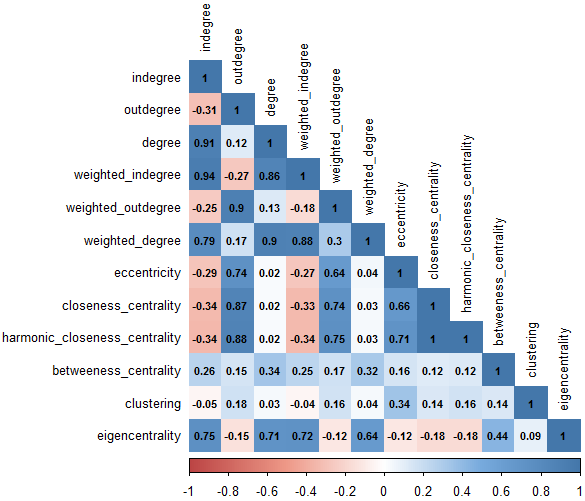
\includegraphics[width=.8\textwidth]{corr-matrix-populism}
\end{figure}
\begin{figure}
  \centering
  \caption{Bivariate correlation matrix for topic: \texttt{refugees}.}\label{corr-matrix-refugees}
  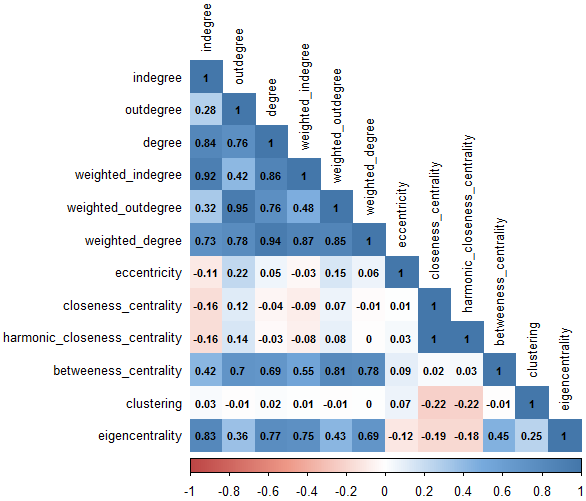
\includegraphics[width=.8\textwidth]{corr-matrix-refugees}
\end{figure}

\clearpage
\begin{figure}
  \centering
  \caption{Bivariate correlation matrix for topic: \texttt{terrorism}.}\label{corr-matrix-terrorism}
  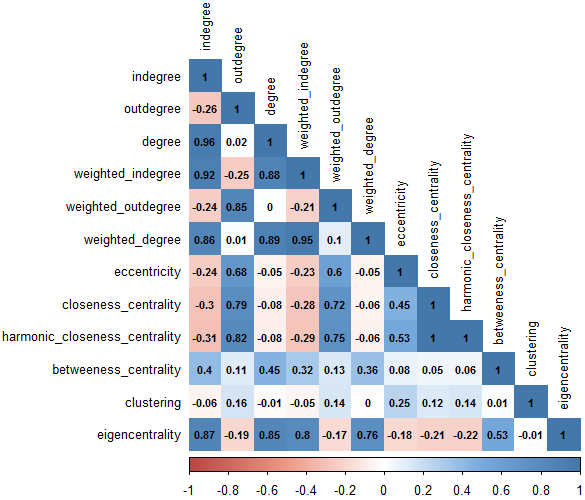
\includegraphics[width=.8\textwidth]{corr-matrix-terrorism}
\end{figure}
\begin{figure}
  \centering
  \caption{Bivariate correlation matrix for topic: \texttt{unemployment}.}\label{corr-matrix-unemployment}
  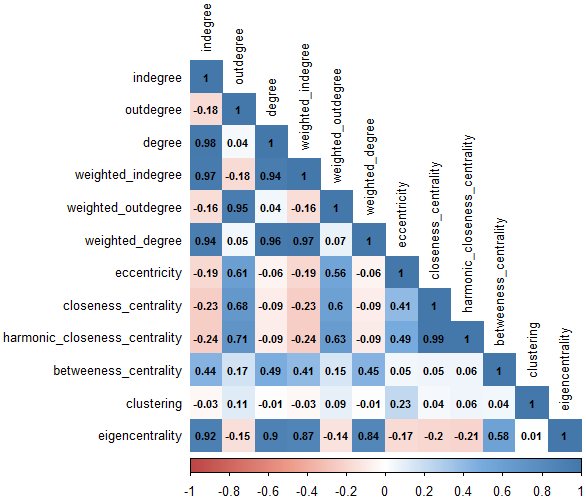
\includegraphics[width=.8\textwidth]{corr-matrix-unemployment}
\end{figure}

\clearpage
\thispagestyle{SectionFirstPage}
\begin{sidewaysfigure}[ht]
  \caption{Coefficients and SE per topic of Model A (Complete OLS).\label{model-a-coeff}}
  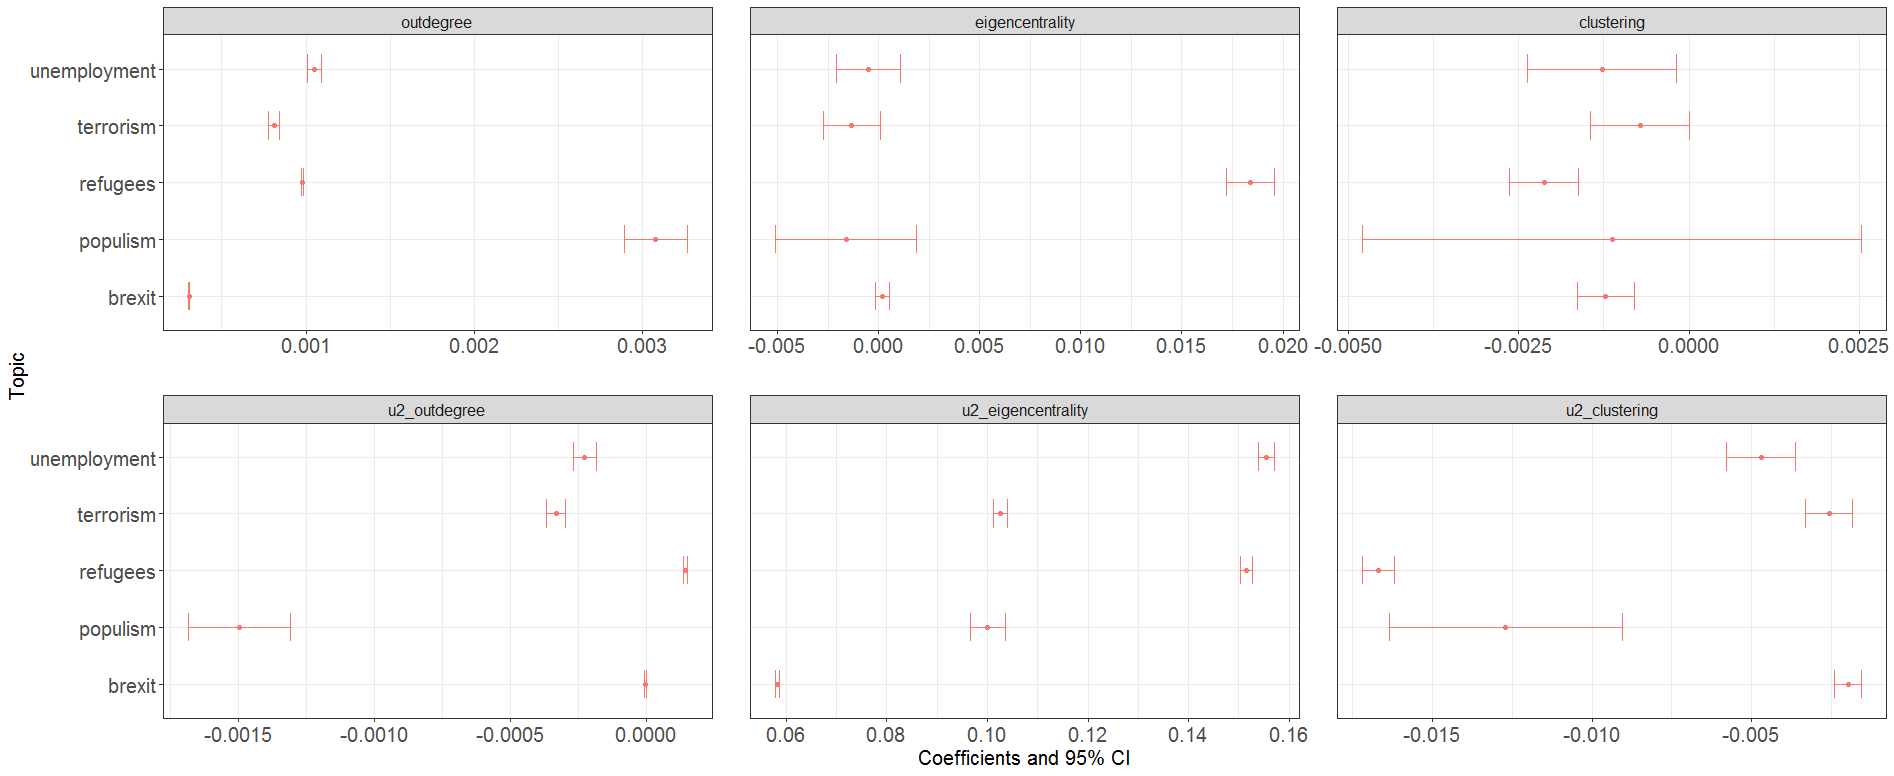
\includegraphics[width=\textwidth]{model_A_coeff}
\end{sidewaysfigure}

\clearpage
\thispagestyle{SectionFirstPage}
\begin{sidewaysfigure}[ht]
  \caption{Coefficients and SE per topic of Model B (Logistic).\label{model-b-coeff}}
  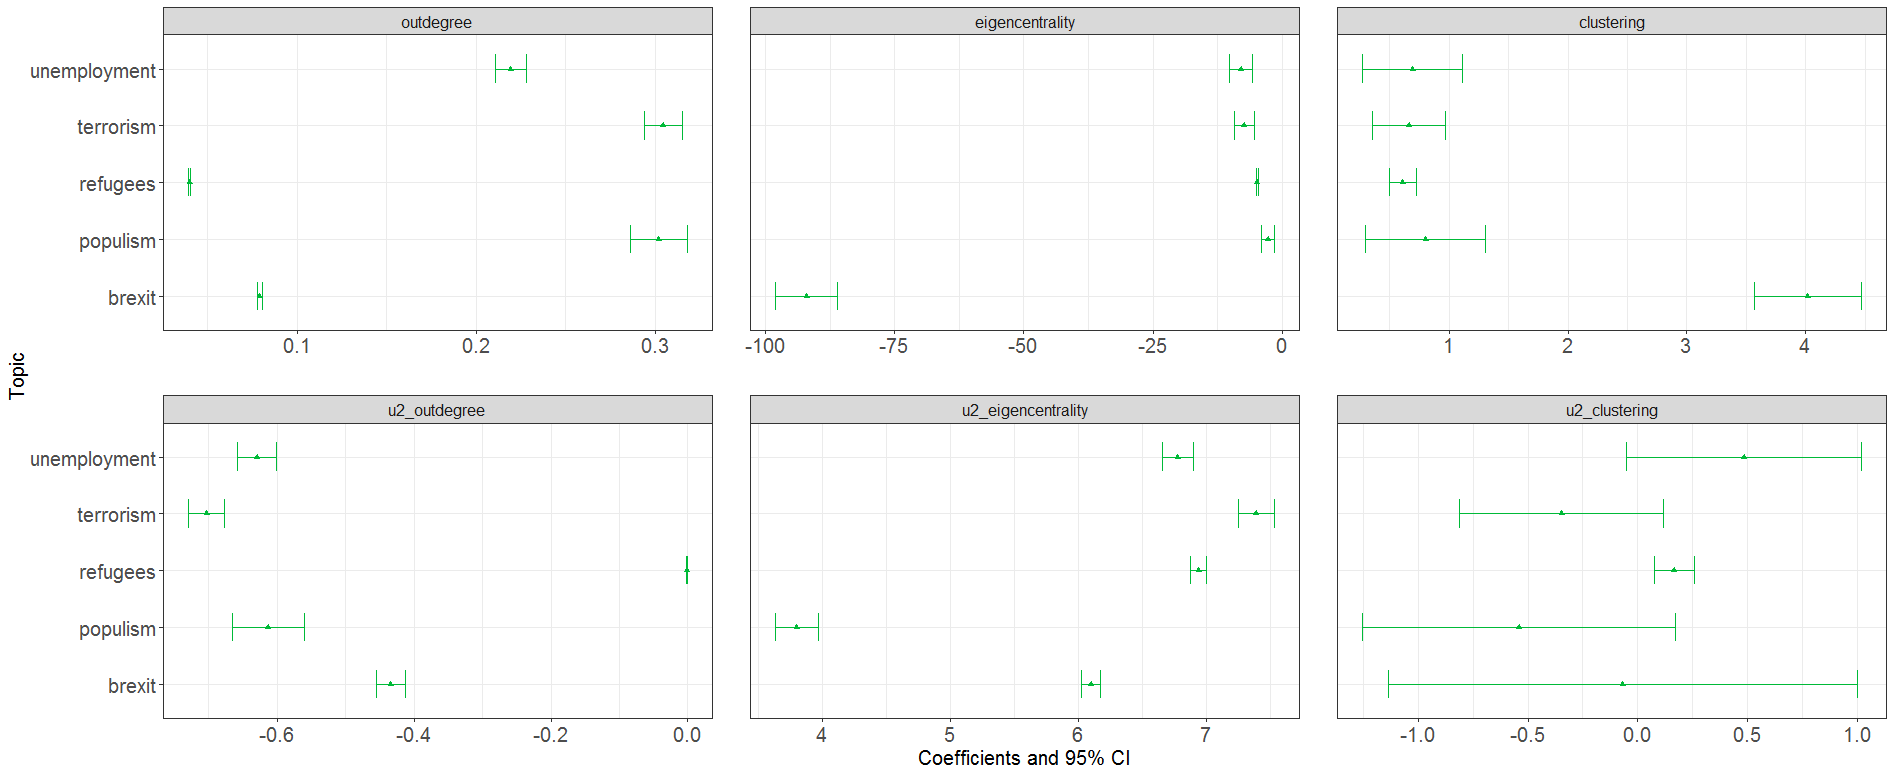
\includegraphics[width=\textwidth]{model_B_coeff}
\end{sidewaysfigure}

\clearpage
\thispagestyle{SectionFirstPage}
\begin{sidewaysfigure}[ht]
  \caption{Coefficients and SE per topic of Model C (Conditional OLS).\label{model-c-coeff}}
  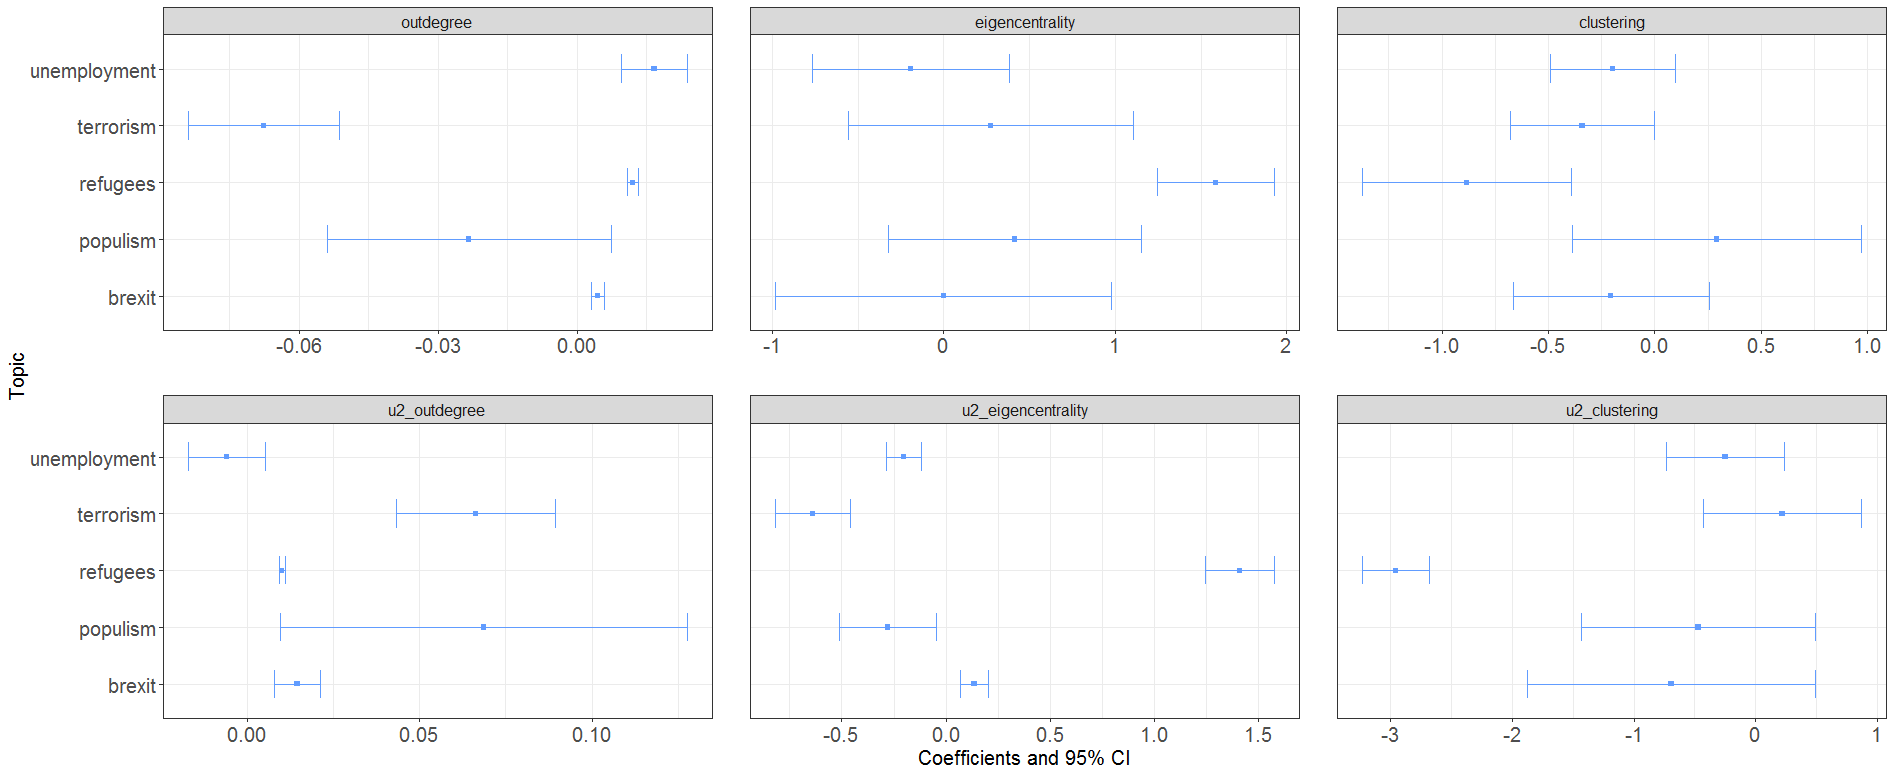
\includegraphics[width=\textwidth]{model_C_coeff}
\end{sidewaysfigure}

\section{Appendix B}\label{appendix-b}\thispagestyle{SectionFirstPage} % Hide headers on the first page of the section
\setcounter{figure}{0}
\setcounter{table}{0}
\obeylines
\begin{multicols}{3}
{\tiny
@volkspartei
@SPOE\_at
@neos\_eu
\#Jetzt
@Gruene\_Austria
\#ListeFirtz
@KPOE\_EL
@vorwaertstirol
\#LBL
@EUNEIN2
@GILTofficial
@PdA\_Austria
@piratenparteiat
@de\_nva
@cdenv
@openvld
@sp\_a
@groen
@vlbelang
@partisocialiste
@mr\_officiel
@lecdh
@ecolo
@defi\_eu
@ppofficiel
@pvdabelgie
@CSPOstbelgien
@PPGERB
@BSP\_Bulgaria
@PatriotiBG
@atakaBG
@HDZ001
@SDPHrvatske
@NLMost
@HSSHrvatska
@HaeNeS\_
@StrankaGLAS
@zivizidhr
@IDSDDI
@BM365\_stranka
@NHRvatsku
@HdsHrvatska
@demokrati\_hr
@NS\_reformisti
@HSLShr
@PromijenimoHR
@HDSSBhr
@DISY
@AKEL1926
@DIKO1976
@KiSos2020
@SymmaxiaPoliton
@allileggii2015
@cygreens
@ELAMcy
@matosmysl
@ODScz
@PiratskaStrana
@SPD\_oficialni
@czKSCM
@CSSD
@kducsl
@TOP09cz
@STANcz
@svobodni
@zeleni\_cz
@Spolitik
@DanskDf1995
@venstredk
@SFpolitik
@KonservativeDK
@Radikale
@Enhedslisten
@LiberalAlliance
@ep14dk
@alternativet\_
@reformikad
@keskerakondlane
@aurorapropatria
@sotsdem
@Demarit
@persut
@kokoomus
@keskusta
@vihreat
@vasemmisto
@sfprkp
@KDpuolue
@enmarchefr
@lesRepublicains
@MoDem
@FranceInsoumise
@PCF
@RNational\_off
@MvtRadical
@LesCentristes\_
@FED\_info
@LGM\_67
@mdPMidiPyrenees
@DLF\_Officiel
@AllianceC
@MRC\_France
@CAP21\_Tweets
@EELV38
@LePG
@GenerationsMvt
@Ensemble\_FdG
@ecologistes\_92
@agir\_officiel
@ComitesJeanne
@ForceDu13
@GenCitoyens
@Liguedusud
@\_LesPatriotes
@Gauche\_RS
@Radicaux2Gauche
@Pe\_A\_Corsica
@PicardieDebout
@cdu
@spdde
@afd
@fdp
@dielinke
@die\_gruenen
@csu
@BlaueWende
@LKR\_Partei\_Bund
@fwlandtag
@oedppresse
@diepartei
@piratenpartei
@npdde
@syriza\_gr
@neademokratia
@kinimallagis
@ToPotami
@anexartitoi
@enosi\_kentroon
@FideszEP
@JobbikMM
@kdnp
@mszptweet
@lehet\_mas
@MLPLiberalisok
@FineGael
@fiannafailparty
@sinnfeinireland
@labour
@solidarityie
@independents4\_C
@greenparty\_ie
@SocDems
@AontuIE
@HumanDignityIre
@RENUAIreland
@workersparty
@Vote4Homes
@RepublicanSF
@Mov5Stelle
@pdnetwork
@LegaSalvini
@forza\_italia
@FratellidItaIia
@liberi\_uguali
@Piu\_Europa
@CasaPoundItalia
@SaskanaOnline
@KamPiederValsts
@konservativie
@AttistibaiPar
@VL\_TBLNNK
@ZZS\_
@Jauna\_Vienotiba
\#LVZS
@tslkd
@lsdp\_vilnius
@darbopartija
@adr\_lu
@CSV\_news
@dp\_lu
@deigreng
@dei\_lenk
@lsap\_lu
@Piratepartei
@PL\_Malta
@PNmalta
@Demokratiku
@vvd
@cdavandaag
@d66
@groenlinks
@spnl
@pvda
@christenunie
@partijvddieren
@50pluspartij
@sgpnieuws
@denknl
@fvdemocratie
@pisorgpl
@Platforma\_org
@KUKIZ15
@nowePSL
@Nowoczesna
@Porozumienie\_\_
@SolidarnaPL
@WolniSolidarni
@wybierz\_TERAZ
@Unia\_Euro\_Dem
@UPR\_org
@PoZdroj
@republikanieorg
@Prawica\_Rz
@RuchNarodowy
@Bialo\_\_Czerwoni
@sldpoland
@NowaPrawica
@OsVerdes
@Blocomadeira
@psocialista
@Partido\_PAN
@LIVREpt
@pdr\_coimbra
@MovimentoJPP
@LiberalPT
@ppdpsd
@\_CDSPP
@Partido\_Alianca
@psdct
@PnlRomania
@usr\_romania
@RMDSZ\_UDMR
@alde\_romania
@smersd
@stranasas
@strankaSDS
@strankaSD
@StrankaSMC
@strankalevica
@NovaSlovenija
@PS\_DeSUS
@StrankaSAB
@SnsStranka
@populares
@PSOE
@ABUnidasPodemos
@CiudadanosCs
@Esquerra\_ERC
@Pdemocratacat
@eajpnv
@PartidoPACMA
@ehbildu
@coalicion
@socialdemokrat
@moderaterna
@sdriks
@miljopartiet
@Centerpartiet
@vansterpartiet
@liberalerna
@kdriks
@Feministerna
@Conservatives
@UKLabour
@theSNP
@LibDems
@ForChange\_Now
@duponline
@Plaid\_Cymru
@TheGreenParty
@scotgp
@brexitparty\_uk
@UKIP
@SDLPlive
@uuponline
@allianceparty
@GreenPartyNI
@pb4p
@TheSDPUK
@sebastiankurz
@rendiwagner
@HCStracheFP
@BMeinl
@Maria\_\_Stern
@WKogler
\#Dinkhauser
\#Kölly
@GabrielHribar
@MarschallRobert
\#RolandDüringer
@bart\_dewever
@wbeke
@ruttengwendolyn
@johncrombez
@meyremalmaci
@tomvangrieken
@eliodirupo
@ochastel
@prevotmaxime
@zakiakhattabi
@oliviermaingain
@modrikamen
@peter\_mertens
@OliverPaasch
@KattrinJadin
@BoykoBorissov
\#KorneliyaNinova
@KKarakachanov
@valeri\_simeonov
@volensiderov
@MareshkiVeselin
@AndrejPlenkovic
@davor\_bernardic
@BozoPetrov
@KBeljak
@anka\_mrak
@Ivan\_Pernar
@\_BorisMiletic
@BrunaEsih
@SilvanoHSU
@drMrsic
@DarinkoKosor
@ladislav\_ilcic
@AverofCY
@GenSecAKEL
@NicholasPapadop
@sizopoulos
@yiorgoslillikas
@THEOCHAROUSE
@gperdikes
@AndrejBabis
@P\_Fiala
@PiratIvanBartos
@tomio\_cz
@vojtafilip
@jhamacek
@MarekVyborny
@Pospisil\_Jiri
@JanFar\_sky
@JTP07
@stepanekpraha
@Kristianthdahl
@larsloekke
@PiaOlsen
@SorenPape
@oestergaard
@PSkipperEL
@anderssamuelsen
@uffeelbaek
@kajakallas
@ratasjuri
@Mart\_Helme
@HelirSeeder
@JevgeniO
@AnttiRinnepj
@Halla\_aho
@PetteriOrpo
@juhasipila
@Haavisto
@liandersson
@anna\_maja
@SariEssayah
@StanGuerini
@laurentwauquiez
@faureolivier
@bayrou
@JLMelenchon
@Fabien\_Rssl
@MLP\_officiel
@LaurentHenart
@Herve\_Morin
@HerveMarseille
@BockelJeanMarie
@RobertHueOff
@dupontaignan
@philippefolliot
@jluc\_laurent
@corinnelepage
@DavidCormand
@ericcoquerel
@benoithamon
@FdeRugy
@jeanlassalle
@franckriester
@lepenjm
@jnguerini
@JeanMarieCAVADA
@JacquesBompard
@f\_philippot
@mnlienemann
@VRoziere
@Gilles\_Simeoni
@Francois\_Ruffin
@akk
@AndreaNahlesSPD
@Joerg\_Meuthen
@c\_lindner
@katjakipping
@ABaerbock
@Markus\_Soeder
@FraukePetry
@Bernd\_Koelmel
@HubertAiwanger
@ChristophRaabs
@MartinSonneborn
@sebulino
@FrankFranz
@atsipras
@kmitsotakis
@IliasKasidiaris
@FofiGennimata
@St\_Theodorakis
@PanosKammenos
@semjen
@GyurcsanyMES
@marta\_demeter
@Bajnai\_Gordon
@LeoVaradkar
@MichealMartinTD
@MaryLouMcDonald
@BrendanHowlin
@EamonRyan
@CathMurphyTD
@Toibin1
@SeamusHealyTD
@RonanMullen
@johnleahyRENUA
@GraTire
@luigidimaio
@nzingaretti
@matteosalvinimi
@berlusconi
@GiorgiaMeloni
@PietroGrasso
@emmabonino
@distefanoTW
@nilsusakovs
@artuss
@Bordans
@pavluts
@RaivisDzintars
@ArmandsKrauze
@aseradens
@RamunasLVZS
@UspaskichV
@Linas\_Balsys
@puteikis
@CorinneCahen
@KmiotekC
@FranzFayot
StarskyFlor
@JosephMuscat\_JM
@adriandeliapn
@GodfreyFarrugia
@markrutte
@geertwilderspvv
@sybrandbuma
@AMSpierings
@jesseklaver
@MarijnissenL
@LodewijkA
@gertjansegers
@mariannethieme
@HenkKrol
@keesvdstaaij
@tunahankuzu
@thierrybaudet
@KaczynskiJaro
@SchetynadlaPO
@pkukiz
@KosiniakKamysz
@KLubnauer
@Jaroslaw\_Gowin
@ZiobroPL
@KornelMorawiec1
@RyszardPetru
@EBinczycka
@BJozwiakUPR
@JkmMikke
@AnnaSiarkowska
@PrawicaKawecki
@wlodekczarzasty
@catarina\_mart
@MadalenoPTP
@ruitavares
@RuiRioPSD
@CristasAssuncao
@PSantanaLopes
@\_LiviuDragnea
@Ludovic\_Orban
@kelemenhunor
@eugen\_tomac
@MonikaFlaBenova
@SulikRichard
@igor\_matovic
@MarianKotleba
@JJansaSDS
@sarecmarjan
@ZidanDejan
@MiroCerar
@LukaMesec
@MatejTonin
@ErjavecKarl
@ABratusek
@ZmagoPlemeniti
@pablocasado\_
@CristinaNarbona
@Pablo\_Iglesias\_
@Albert\_Rivera
@junqueras
@davidbonvehi
@andoniortuzar
@ArnaldoOtegi
@anioramas
@SwedishPM
@ulfgooglar
@jimmieakesson
@bolund
@annieloof
@jsjostedt
@bjorklundjan
@BuschEbba
@gudschy
@theresa\_may
@jeremycorbyn
@NicolaSturgeon
@joswinson
@heidiallen75
@DUPleader
@Adamprice
@jon\_bartley
@patrickharvie
@Nigel\_Farage
@GerardBattenMEP
@columeastwood
@RobinSwannUUP
@naomi\_long
@ClareBaileyGPNI
@JimAllister
@WilliamClouston
\#eurovaalit2019
\#EUvaalit2019
\#ElezioniEuropee
\#ElezioniEuropee2019
\#EP2019
\#EU2019
\#EuropeanElections
\#EuropeanElection2019
\#Europawahl2019
\#Europeias2019
\#Europa2019
\#Europawahl
\#EUverkiezingen
\#EuropeseVerkiezingen
\#EUelections2019
\#EP19
\#ALDE
\#EPP
\#S\&D
\#ECR
\#GUENGL
\#Greens
\#EFA
\#EFDD
\#ENF
@ALDEgroup
@EPP
@TheProgressives
@ecrgroup
@GUENGL
@GreensEP
@EFDgroup
@ENF\_EP
@EFAparty
@EPPGroup
brexit
refugees
flóttamenn
bēgļi
pabėgėliams
flyktninger
uchodźcy
refugiados
refugiați
\textcyr{избеглице}
utečenci
beguncev
flyktingar
ffoaduriaid
immigrati
\textcyr{бежанци}
uprchlíků
flygtninge
vluchtelingen
põgenikele
pakolaisten
immigrés
Flüchtlinge
\begin{otherlanguage*}{greek}
πρόσφυγες
\end{otherlanguage*}
menekültek
terrorism
hryðjuverk
terorismu
terorizmas
terrorisme
terroryzm
terrorismo
terorism
\textcyr{тероризам}
terorizmus
terorizma
terfysgaeth
\textcyr{тероризъм}
terorismus
terrorismiga
terrorismi
Terrorismus
\begin{otherlanguage*}{greek}
τρομοκρατία
\end{otherlanguage*}
terrorizmus
public debt
skuldir hins opinbera
valsts parāds
valstybės skola
offentlig gjeld
dług publiczny
dívida pública
datorie publica
\textcyr{Јавни дуг}
verejný dlh
javni dolg
deuda publica
statsskuld
dyled gyhoeddus
debito pubblico
\textcyr{публичен дълг}
veřejný dluh
offentlig gæld
Publieke schuld
riigivõlg
julkinen velka
dette publique
Staatsverschuldung
\begin{otherlanguage*}{greek}
δημόσιο χρέος
\end{otherlanguage*}
államadósság
single market
innri markaðurinn
vienoto tirgu
bendroji rinka
indre marked
jednolity rynek
mercado único
piață unică
\textcyr{јединствено тржиште}
jednotného trhu
enotnega trga
Enskild marknad
marchnad sengl
mercato comune europeo
\textcyr{Единен пазар}
Jednotný trh
Interne markt
Ühtne turg
Sisämarkkinat
marché unique
Binnenmarkt
\begin{otherlanguage*}{greek}
ενιαία αγορά
\end{otherlanguage*}
egységes piacon
gender equality
jafnrétti kynjanna
dzimumu līdztiesība
lyčių lygybė
Likestilling
równość płci
igualdade de gênero
egalitatea sexelor
\textcyr{родна равноправност}
rovnosť pohlaví
enakost med spoloma
igualdad de género
jämställdhet mellan könen
Cydraddoldeb Rhyw
uguaglianza di genere
\textcyr{равенството между половете}
rovnosti žen a mužů
ligestilling
geslachtsgelijkheid
sooline võrdõiguslikkus
sukupuolten tasa-arvo
égalité des sexes
Geschlechtergleichheit
\begin{otherlanguage*}{greek}
ισότητα των φύλων
\end{otherlanguage*}
nemek közötti egyenlőség
lgbt rights
lgbt réttindi
lgbt tiesības
Lgbt teisės
lgbt rettigheter
prawa LGBT
direitos lgbt
Lgbt drepturile
\textcyr{лгбт ригхтс}
lgbt práva
lgbt pravice
derechos lgbt
lgbt rättigheter
hawliau LHDT
diritti lgbt
\textcyr{lgbt права}
práva lgbt
lgbt rettigheder
lgbt rechten
LGBT õiguste
lgbt-oikeudet
lgbt droits
lgbt Rechte
\begin{otherlanguage*}{greek}
lgbt δικαιώματα
\end{otherlanguage*}
lgbt jogok
unemployment
atvinnuleysi
bezdarbs
nedarbas
arbeidsledighet
bezrobocie
desemprego
şomaj
\textcyr{незапослености}
nezamestnanosť
brezposelnosti
desempleo
arbetslöshet
diweithdra
disoccupazione
\textcyr{безработица}
nezaměstnanost
arbejdsløshed
werkloosheid
tööpuudus
työttömyys
chômage
Arbeitslosigkeit
\begin{otherlanguage*}{greek}
ανεργία
\end{otherlanguage*}
munkanélküliség
populism
populisms
populizmas
populisme
populizm
populismo
\textcyr{популизам}
populizmus
populizem
\textcyr{популизъм}
populismus
populismi
\begin{otherlanguage*}{greek}
λαϊκισμού
\end{otherlanguage*}
fake news
eu institutions
eu stofnanir
Eiropas Savienības iestādes
Europos Sąjungos institucijos
europeiske union institusjoner
instytucje unii europejskiej
instituições da união europeia
instituțiile Uniunii Europene
\textcyr{институције европске уније}
inštitúcie EÚ
institucij eu
intituciones de la ue
eu institutioner
sefydliadau r UE
istituzioni europee
\textcyr{институции Европейския съюз}
instituce Evropské unie
instellingen van de Europese Unie
Euroopa Liidu institutsioonid
Euroopan unionin toimielimet
institutions européennes
eu institutionen
EU-intézmények
\begin{otherlanguage*}{greek}
θεσμικά όργανα της ΕΕ
\end{otherlanguage*}}
\end{multicols}


\end{document}
